\documentclass[a4paper,11pt]{book}
\usepackage{listings}
\usepackage[utf8]{inputenc}
\usepackage[spanish]{babel}


\decimalpoint
\usepackage{dcolumn}
\newcolumntype{.}{D{.}{\esperiod}{-1}}
\makeatletter
\addto\shorthandsspanish{\let\esperiod\es@period@code}
\makeatother


\RequirePackage{verbatim}
\usepackage{fancyhdr}
\usepackage{graphicx}
\usepackage{afterpage}
\usepackage{tabularx}
\usepackage{float}

\usepackage{longtable}
\usepackage[hyphens]{url}
\usepackage[pdfborder={0 0 0}]{hyperref} %referencia

% ********************************************************************
% Re-usable information
% ********************************************************************
\newcommand{\myTitle}{Aplicación web gestión de entrenamientos\xspace}
\newcommand{\myDegree}{Grado en Ingeniería Informática\xspace}
\newcommand{\myName}{Antonio de la Vega Jiménez\xspace}
\newcommand{\myProf}{Juan Julián Merelo Guervós\xspace}

\newcommand{\mySupervisor}{Juan Julián Merelo Guervós\xspace}
\newcommand{\myFaculty}{Escuela Técnica Superior de Ingenierías Informática y de
Telecomunicación\xspace}
\newcommand{\myFacultyShort}{E.T.S. de Ingenierías Informática y de
Telecomunicación\xspace}
\newcommand{\myDepartment}{Departamento de Arquitectura de Computadores\xspace}
\newcommand{\myUni}{\protect{Universidad de Granada}\xspace}
\newcommand{\myLocation}{Granada\xspace}
\newcommand{\myTime}{\today\xspace}
\newcommand{\myVersion}{Version 0.1\xspace}


\hypersetup{
pdfauthor = {\myName (antoniovj1@correo.ugr.es)},
pdftitle = {\myTitle},
pdfsubject = {},
pdfkeywords = {Web, Node.js, React.js, MongoDB, Integración continua, Despliegue continuo},
pdfcreator = {LaTeX},
pdfproducer = {pdflatex}
}

\usepackage{colortbl,longtable}
\usepackage[stable]{footmisc}


\pagestyle{fancy}
\fancyhf{}
\fancyhead[LO]{\leftmark}
\fancyhead[RE]{\rightmark}
\fancyhead[RO,LE]{\textbf{\thepage}}
\renewcommand{\chaptermark}[1]{\markboth{\textbf{#1}}{}}
\renewcommand{\sectionmark}[1]{\markright{\textbf{\thesection. #1}}}

\setlength{\headheight}{1.5\headheight}

\newcommand{\HRule}{\rule{\linewidth}{0.5mm}}

\definecolor{gray97}{gray}{.97}
\definecolor{gray75}{gray}{.75}
\definecolor{gray45}{gray}{.45}
\definecolor{gray30}{gray}{.94}

\lstset{ frame=Ltb,
     framerule=0.5pt,
     aboveskip=0.5cm,
     framextopmargin=3pt,
     framexbottommargin=3pt,
     framexleftmargin=0.1cm,
     framesep=0pt,
     rulesep=.4pt,
     backgroundcolor=\color{gray97},
     rulesepcolor=\color{black},
     %
     stringstyle=\ttfamily,
     showstringspaces = false,
     basicstyle=\scriptsize\ttfamily,
     commentstyle=\color{gray45},
     keywordstyle=\bfseries,
     %
     numbers=left,
     numbersep=6pt,
     numberstyle=\tiny,
     numberfirstline = false,
     breaklines=true,
   }
 
% minimizar fragmentado de listados
\lstnewenvironment{listing}[1][]
   {\lstset{#1}\pagebreak[0]}{\pagebreak[0]}

\lstdefinestyle{CodigoC}
   {
	basicstyle=\scriptsize,
	frame=single,
	language=C,
	numbers=left
   }
\lstdefinestyle{CodigoC++}
   {
	basicstyle=\small,
	frame=single,
	backgroundcolor=\color{gray30},
	language=C++,
	numbers=left
   }

 
\lstdefinestyle{Consola}
   {basicstyle=\scriptsize\bf\ttfamily,
    backgroundcolor=\color{gray30},
    frame=single,
    numbers=none
   }


\newcommand{\bigrule}{\titlerule[0.5mm]}


\makeatletter
\def\clearpage{
  \ifvmode
    \ifnum \@dbltopnum =\m@ne
      \ifdim \pagetotal <\topskip
        \hbox{}
      \fi
    \fi
  \fi
  \newpage
  \thispagestyle{empty}
  \write\m@ne{}
  \vbox{}
  \penalty -\@Mi
}
\makeatother

\usepackage{pdfpages}




\definecolor{lightgray}{rgb}{.9,.9,.9}
\definecolor{darkgray}{rgb}{.4,.4,.4}
\definecolor{purple}{rgb}{0.65, 0.12, 0.82}

\lstdefinelanguage{JavaScript}{
  keywords={typeof, new, true, false, catch, async, await, function, return, null, catch, switch, var, if, in, while, do, else, case, break},
  keywordstyle=\color{blue}\bfseries,
  ndkeywords={class, export, boolean, throw, implements, import, this},
  ndkeywordstyle=\color{darkgray}\bfseries,
  identifierstyle=\color{black},
  sensitive=false,
  comment=[l]{//},
  morecomment=[s]{/*}{*/},
  commentstyle=\color{purple}\ttfamily,
  stringstyle=\color{red}\ttfamily,
  morestring=[b]',
  morestring=[b]"
}

\lstset{
   language=JavaScript,
   backgroundcolor=\color{lightgray},
   extendedchars=true,
   basicstyle=\footnotesize\ttfamily,
   showstringspaces=false,
   showspaces=false,
   numbers=left,
   numberstyle=\footnotesize,
   numbersep=9pt,
   tabsize=2,
   breaklines=true,
   showtabs=false,
   captionpos=b
}

\usepackage[table,xcdraw]{xcolor} 
\usepackage{graphicx}
\usepackage[toc,title,page]{appendix}
\usepackage[toc,style=altlistgroup]{glossaries}

\makeglossaries
\newglossaryentry{git}
{
name={git},
description={definición}
}
\newglossaryentry{DevOps}
{
name={DevOps},
description={definición}
}
\newglossaryentry{microciclo}
{
name={microciclo},
description={definición}
}
\newglossaryentry{backend}
{
name={backend},
description={definición}
}
\newglossaryentry{frontend}
{
name={frontend},
description={definición}
}

\newglossaryentry{API}
{
name={API},
description={definición}
}

\newglossaryentry{Integracion continua}
{
name={Integración continua},
description={definición}
}

\newglossaryentry{Despliegue continuo}
{
name={Despliegue continuo},
description={definición}
}

\newglossaryentry{Test de cobertura}
{
name={Test de cobertura},
description={definición}
}

\newglossaryentry{Test unitarios}
{
name={Test unitarios},
description={definición}
}

\newglossaryentry{test A/B}
{
name={test A/B},
description={definición}
}

\newglossaryentry{provisionamiento}
{
name={provisionamiento},
description={definición}
}

\newglossaryentry{NPM}
{
name={NPM},
description={definición}
}

\newglossaryentry{material design}
{
name={material design},
description={definición}
}

\newglossaryentry{push}
{
name={push},
description={definición}
}

\newglossaryentry{No-SQL}
{
name={No-SQL},
description={definición}
}

\newglossaryentry{middleware}
{
name={middleware},
description={definición}
}

\newglossaryentry{endpoint}
{
name={endpoint},
description={definición}
}

\newglossaryentry{pull request}
{
name={pull request},
description={definición}
}

\newglossaryentry{merge}
{
name={merge},
description={definición}
}

\newglossaryentry{SPA}
{
name={SPA},
description={definición}
}

\newglossaryentry{RESTful}
{
name={RESTful},
description={definición}
}

\newglossaryentry{logging}
{
name={logging},
description={definición}
}

\newglossaryentry{BSON}
{
name={BSON},
description={definición}
}

\newglossaryentry{JSON}
{
name={JSON},
description={definición}
}

\newglossaryentry{JSX}
{
name={JSX},
description={definición}
}

\newglossaryentry{ODM}
{
name={ODM},
description={definición}
}

\newglossaryentry{driver}
{
name={driver},
description={definición}
}

\newglossaryentry{pseudojoins}
{
name={pseudojoins},
description={definición}
}

\newglossaryentry{orquestacion}
{
name={orquestación},
description={definición}
}

\newglossaryentry{bundle}
{
name={bundle},
description={definición}
}

\newglossaryentry{proxy inverso}
{
name={proxy inverso},
description={definición}
}

\newglossaryentry{hooks}
{
name={hooks},
description={definición}
}

\newglossaryentry{linter}
{
name={linter},
description={definición}
}

\newglossaryentry{PaaS}
{
name={PaaS},
description={definición}
}

\newglossaryentry{build}
{
name={build},
description={definición}
}

\newglossaryentry{Full Stack}
{
name={Full Stack},
description={definición}
}



\begin{document}
\begin{titlepage}
 
 
\newlength{\centeroffset}
\setlength{\centeroffset}{-0.5\oddsidemargin}
\addtolength{\centeroffset}{0.5\evensidemargin}
\thispagestyle{empty}

\noindent\hspace*{\centeroffset}\begin{minipage}{\textwidth}

\centering

\includegraphics[width=0.9\textwidth]{imagenes/logo_ugr.jpg}\\[1.4cm]

\textsc{ \Large TRABAJO FIN DE GRADO\\[0.2cm]}
\textsc{ INGENIERÍA EN INFORMÁTICA}\\[1cm]
% Upper part of the page
% 
% Title
{\Huge\bfseries Aplicación Gestión Entrenamiento\\
}
\noindent\rule[-1ex]{\textwidth}{3pt}\\[3.5ex]
{\large\bfseries Aplicación web con tecnologías modernas}
\end{minipage}

\vspace{1cm}
\noindent\hspace*{\centeroffset}\begin{minipage}{\textwidth}
\centering

\textbf{Autor}\\ {Antonio de la Vega Jiménez}\\[2.5ex]
\textbf{Director}\\
{Juan Julián Merelo Guervós\\[0.5cm] }

\includegraphics[width=0.3\textwidth]{imagenes/etsiit_logo.png}\\[0.1cm]
\textsc{Escuela Técnica Superior de Ingenierías Informática y de Telecomunicación}\\
\textsc{---}\\
Granada, Junio de 2018


\includegraphics[width=0.3\textwidth]{imagenes/CC-SA-logo.png}
\end{minipage}
%\addtolength{\textwidth}{\centeroffset}
%\vspace{\stretch{2}}
\end{titlepage}

\chapter*{}
%\thispagestyle{empty}
%\cleardoublepage

%\thispagestyle{empty}

\begin{titlepage}
 
 
\setlength{\centeroffset}{-0.5\oddsidemargin}
\addtolength{\centeroffset}{0.5\evensidemargin}
\thispagestyle{empty}

\noindent\hspace*{\centeroffset}\begin{minipage}{\textwidth}

\centering
%
\includegraphics[width=0.9\textwidth]{imagenes/logo_ugr.jpg}\\[1.4cm]

%\textsc{ \Large PROYECTO FIN DE CARRERA\\[0.2cm]}
%\textsc{ INGENIERÍA EN INFORMÁTICA}\\[1cm]
% Upper part of the page
% 

 \vspace{3.3cm}

%si el proyecto tiene logo poner aquí

\includegraphics[width=0.3\textwidth]{imagenes/logo.png} 
 \vspace{0.5cm}

% Title

{\Huge\bfseries Aplicación Gestión Entrenamientos\\
}
\noindent\rule[-1ex]{\textwidth}{3pt}\\[3.5ex]
{\large\bfseries Aplicación web con tecnologías modernas.\\[4cm]}
\end{minipage}

\vspace{2.5cm}
\noindent\hspace*{\centeroffset}\begin{minipage}{\textwidth}
\centering

\textbf{Autor}\\ {Antonio de la Vega Jiménez}\\[2.5ex]
\textbf{Director}\\
{Juan Julián Merelo Guervós\\[2cm] }
%
\includegraphics[width=0.15\textwidth]{imagenes/tstc.png}\\[0.1cm]
%\textsc{Departamento de Teoría de la Señal, Telemática y Comunicaciones}\\
%\textsc{---}\\
%Granada, mes de 201
\end{minipage}
%\addtolength{\textwidth}{\centeroffset}
\vspace{\stretch{2}}

 
\end{titlepage}




\cleardoublepage
\thispagestyle{empty}

\begin{center}
{\large\bfseries Aplicación Gestión Entrenamientos: Aplicación web con tecnologías modernas}\\
\end{center}
\begin{center}
Antonio de la Vega Jiménez\\
\end{center}

%\vspace{0.7cm}
\noindent{\textbf{Palabras clave}: Web, Node.js, React.js, MongoDB, Integración continua, Despliegue continuo}\\

\vspace{0.7cm}
\noindent{\textbf{Resumen}}\\

Se pretende desarrollar una plataforma web que simplifique el seguimiento de entrenamientos de pesas, proporcionando a los usuarios la información necesaria para llevar un seguimiento sobre la progresión de las cargas a lo largo del tiempo, así como unas estadísticas indicando sobre que grupos musculares se ha hecho mas énfasis y con ello poder evitar estancamientos, descompensaciones y con ello lesiones causadas por una mala progresión.

El objetivo de este desarrollo es crear una plataforma web basada en código libre, que pueda ser usada por cualquier club deportivo así como por cualquier particular, de forma gratuita y con la posibilidad de ser editada para adaptarse a las necesidades de los usuarios.


Para la construcción de este proyecto se hará uso del sistema de control de versiones GIT, el cual nos permite un desarrollo colaborativo y organizado. Además para obtener un software de calidad y fácilmente desplegable, se utilizaran herramientas para:
\begin{itemize}
  \item Tecnologías modernas.
  \item Realizar provisionamiento gestión de la infraestructura.
  \item Validación mediante tests unitarios
  \item Comprobación de la calidad del código y conflictos mediante integración continua.
  \item Actualizaciones rápidas sin interrupciones mediante despliegue continuo.
\end{itemize}

A lo largo del desarrollo se utilizaran ciertas tecnologías para programación elegidas meticulosamente, en el servidor se usara Node.js junto a Express y una base de datos MongoDB, lo cual nos permitirá un desarrollo ágil y nos dará la capacidad de realizar modificaciones sin un coste de trabajo excesivamente alto. En el lado del cliente se usara React.js junto a Redux, que nos permitirá crear una interfaz basada en componentes reutilizables con un estado global, lo cual nos lleva a crear un código mas fácilmente testeable, mantenible y reutilizable. Para apoyar el desarrollo, se hará uso de herramientas como Jest, TravisCI, Ansible y Docker, de las cuales se hablará en detalle posteriormente.

\cleardoublepage


\thispagestyle{empty}


\begin{center}
{\large\bfseries Web App for gym training management: Web App using modern technologies}\\
\end{center}
\begin{center}
Antonio, De la Vega\\
\end{center}

%\vspace{0.7cm}
\noindent{\textbf{Keywords}: Web, Node.js, React.js, MongoDB, Continuous Integration, Continuous Deployment}\\

\vspace{0.7cm}
\noindent{\textbf{Abstract}}\\

The aim is to develop a web platform that simplifies the monitoring of weight training, providing users with the necessary information to track the progression of loads over time, as well as statistics indicating which muscle groups have been made more emphasis and with it to be able to avoid stagnation, decompensation and with it injuries caused by a bad progression.

The objective of this development is to create a web platform based on free code, which can be used by any sports club as well as by any individual, free of charge and with the possibility of being edited to adapt to the needs of users.

\chapter*{}
\thispagestyle{empty}

\noindent\rule[-1ex]{\textwidth}{2pt}\\[4.5ex]

Yo, \textbf{Antonio de la Vega Jiménez}, alumno de la titulación Grado en Ingeniería Informática de la \textbf{Escuela Técnica Superior
de Ingenierías Informática y de Telecomunicación de la Universidad de Granada}, con DNI XXXXXXXXX, autorizo la
ubicación de la siguiente copia de mi Trabajo Fin de Grado en la biblioteca del centro para que pueda ser
consultada por las personas que lo deseen.

\vspace{6cm}

\noindent Fdo: Antonio de la Vega Jiménez

\vspace{2cm}

\begin{flushright}
Granada a 17 de junio de 2018 .
\end{flushright}


\chapter*{}
\thispagestyle{empty}

\noindent\rule[-1ex]{\textwidth}{2pt}\\[4.5ex]

D. \textbf{Juan Julián Merelo Guervós}, Profesor del Área de XXXX del Departamento YYYY de la Universidad de Granada.

\vspace{0.5cm}

\textbf{Informan:}

\vspace{0.5cm}

Que el presente trabajo, titulado \textit{\textbf{Aplicación Gestión Entrenamientos: Aplicación web con tecnologías modernas}},
ha sido realizado bajo su supervisión por \textbf{Antonio de la Vega Jimémez}, y autorizamos la defensa de dicho trabajo ante el tribunal
que corresponda.

\vspace{0.5cm}

Y para que conste, expiden y firman el presente informe en Granada a X de mes de 2018 .

\vspace{1cm}

\textbf{Los directores:}

\vspace{5cm}

\noindent \textbf{Antonio de la Vega Jiménez \ \ \ \ \ }

\chapter*{Agradecimientos}
\thispagestyle{empty}

       \vspace{1cm}


A todos.


\frontmatter
\tableofcontents
\listoffigures
\listoftables

\mainmatter
\setlength{\parskip}{5pt}


\chapter{Introducción}
En la actualidad el levantamiento de pesas es un tipo de entrenamiento ampliamente realizado, debido a que se conoce que puede aportar grandes beneficios a la salud, aunque si es realizado sin precaución se pueden producir lesiones, ya sea por una progresión mal planificada, una mala técnica de levantamiento, una mala nutrición o un déficit de descanso. Una de las tareas más sencillas para evitar lesiones, es observar la evolución de la progresión, buscando estancamientos o progresos demasiado rápidos. Por otro lado una tarea a realizar algo más compleja es el seguimiento de la carga aplicada por sesión de entrenamiento y grupo muscular.

Durante años practicando deporte he observado que la mayoría de deportistas amateur, se centran en la nutrición y la técnica, pero no prestan suficiente atención a la progresión, limitándose a cargar el máximo posible, o a la generación de desequilibrios musculares. 

En mi experiencia, este seguimiento no se realiza debido al desconocimiento la importancia de esta tarea, al desconocimiento de las progresiones basadas en ciclos y microciclos, a la complejidad de saber los músculos implicados en cada ejercicio, o simplemente a la pereza de llevar a cabo dicho seguimiento.

Debido a esas observaciones me propuse realizar una aplicación Web que de forma sencilla permite monitorizar el progreso y el uso de los diferentes grupos musculares, con lo cual, proporcionar una serie de datos con los que ayudar a un usuario a obtener sus propias conclusiones.

Dicho esto, cabe destacar que la aplicación simplemente proporcionará datos objetivos sobre la progresión y los grupos musculares usados, y que de ningún modo proporciona ningún consejo, esto se debe a que la planificación de un entrenamiento conlleva una gran complejidad, ya que cada individuo tiene sus propias características y esta tarea debe ser realizada por una profesional dada su implicación en la salud.

Para la implementación de este proyecto se llevará a cabo una metodología DevOps, que quedará detallada en los capítulos 5 (Diseño) en el cual se explicaran las decisiones tomadas y 6 (Implementación) en el cual se mostrará como se ha llevado a cabo el desarrollo.

Por otro lado en los próximos tres capítulos ( Especificación de requisitos, Planificación y Análisis ), se mostrará que requisitos debe cumplir la aplicación para que pueda llevar a cabo su cometido, como se planificó el desarrollo del software a lo largo del tiempo y un análisis detallado de todo lo anterior.

Finalmente existen dos capítulos adicionales, en primer lugar el 7, en el que detallaremos los tests realizados sobre el software, tanto sobre la calidad del código, como sobre el buen funcionamiento de la aplicaciónes, tras esto se incluye un último capítulo donde se abordarán las conclusiones y la evolución futura de la aplicación.

%
\chapter{Especificación Requisitos}
%
\chapter{Planificación}

\section {Fases y entregas}
\subsection {Fases}

Este proyecto estará compuesto por seis fases, cobrando un gran peso en tiempo tres de ellas, la Análisis y diseño, la Implementación ( aunque se parta de una base de código iniciada con anterioridad) y la de pruebas, todas las fases serán las siguientes:

\begin{itemize}
  \item Fase 1: Especificaciones del proyecto.
  \item Fase 2: Planificación.
  \item Fase 3: Análisis y diseño.
  \item Fase 4: Desarrollo.
\end{itemize}

\subsection {Lista de actividades}
A continuación se muestra las actividades a desarrollar en cada fase. Como se puede observar, debido a nuestra orientación DevOps, una vez que en las primeras fases hemos conseguido una idea relativamente definida, pero no final, sobre la que podemos sentar las bases del proyecto , comenzamos una cuarta fase, en la cual se llevan en paralelo y de forma incremental varias tareas, como son la implementación, la documentación y las pruebas, pruebas que representan la especificación.

\begin{itemize}
  \item Fase 1: Especificaciones del proyecto.
    \begin{enumerate}
      \item Determinación objetivos.
      \item Determinación requisitos.
    \end{enumerate}
  \item Fase 2: Planificación.
    \begin{enumerate}
      \item Lista de actividades
      \item Entrevistas
      \item Presupuesto
    \end{enumerate}
  \item Fase 3: Análisis y diseño.
    \begin{enumerate}
      \item Análisis de requisitos
      \item Diagramas
      \item Metodología de desarrollo.
      \item Descripción estructural
    \end{enumerate}
  \item Fase 4: Desarrollo.
    \begin{itemize}
       \item \textbf{Implementación:} 
       \begin{itemize}
         \item  Infraestructura.
         \item  Base de datos.
         \item  Backend.
         \item  Fronted.
       \end{itemize}
       \item \textbf{Pruebas:} 
       \begin{itemize}
        \item  \gls{Test unitarios}.
        \item  \gls{Test de cobertura}.
        \item  \gls{Integracion continua}.
        \item  \gls{Despliegue continuo}.
       \end{itemize}
       \item \textbf{Documentación:} 
       \begin{itemize}
        \item  API/BackEnd.
        \item  FrontEnd.
        \item  Proyecto.
       \end{itemize}
    \end{itemize}
\end{itemize}

En la siguiente imagen \ref{fig:gantt}, se muestra un diagrama de Gantt con la planificación seguida.

\begin{figure}
  \begin{center}
    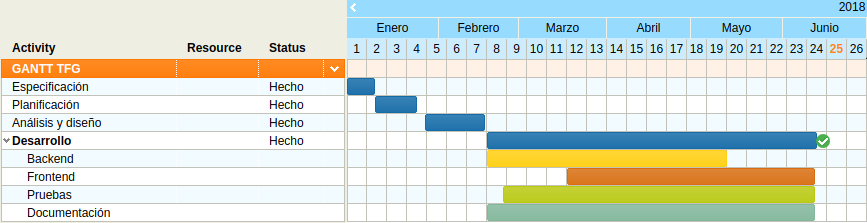
\includegraphics[width=\textwidth]{imagenes/gantt.png}
    \caption{Diagrama de Gantt}
    \label{fig:gantt}
  \end{center}
\end{figure}



\section {Entrevistas}
Para poder alcanzar una interfaz cómoda y de calidad, se ha realizado una serie de preguntas un \gls{test A/B} a varios usuarios, de forma que usando el feedback proporcionado se han tomado las decisiones para la forma en la que se introducen y se muestran los datos.

\section {Presupuestos}

Para este proyecto se ha utilizado software libre y versiones gratuitas de ciertas plataformas como Auth0, TravisCI, GitHub, GreenKeeper, SonnarQube, mLab, PaperTrail y Heroku entre otras. Por ello el coste en licencias en infraestructura de desarrollo es nulo. Cabe destacar que se han realizado despliegues en Google Cloud, que aunque se ha realizado haciendo uso de créditos gratuitos, si que conllevaría un gasto si se optara por mantener la aplicación en dicha plataforma.
En caso de querer realizar un despliegue permanente mencionado anteriormente y  suponiendo 7000 usuarios mensuales activos, el precio de la autenticación seguiría siendo gratuito aunque
por otro lado está el coste de la infraestructura. Debido a que la mayor parte de la computación
se hace en el lado del cliente, no se requiere un hardware de gran potencia, por ello optamos por
una máquina con 3.75Gb de RAM, 200GB de almacenamiento, 1 CPU y 456 horas de uso real al mes, lo cual, alojado en Google Cloud, nos costaría un total de 22,11\euro  al mes. Al margen de los costes de infraestructura y licencia, también se debe tener en cuenta el precio del desarrollo, con un tiempo  de 400 horas de trabajo y suponiendo un salario de 12\euro  la hora, habría que valorar en 4800\euro .

%
\chapter{Análisis}

\section {Actores}
En este analisis nos encontraremos con dos actores, el usuario y el desarrollador.

El desarrolador sera el encargado del mantenimiento, administracion y evolución de la aplicacion, por ello será una persona con conocimientos tecnicos que haga trabajos de progrmación y de administración de la infraestructura.

El usuario, será cualquier persona que desee mantener un registro de sus entrenamientos, este actor no requerirá de conocimientos tecnicos, pero si que se presupondra que tiene los conocimientos basiscos para interacturar con un navegador web.

Estos dos actores son una generalización de todos los posibles usuarios que pueden usar la aplicación, desde los diferentes puntos de vista posibles.

\section{Especificación de requisitos}

En esta sescion se detallan los requisitos que debe cumplimentar el software desarrollado para garantizar que cumple su proposito y con ello que cubre la necesidad para la que ha sido creado.

\subsection{Requisitos Funcionales}

\begin{itemize}
  \item \textbf{RF-1.} Gestión de usuarios.
  \begin{itemize}
    \item \textbf{RF-1.1.} Alta de usuarios.
    \item \textbf{RF-1.2.} Autenticación usuarios.
    \begin{itemize}
      \item \textbf{RF-1.2.1.} Acceso social (Google, Facebook...)
      \item \textbf{RF-1.2.2.} Recordatorio contraseña.
      \item \textbf{RF-1.2.3.} Verificación de email.
    \end{itemize}
    \item \textbf{RF-1.3.} Baja usuarios.
    \item \textbf{RF-1.4.} Edición perfil usuarios
  \end{itemize}
  \item \textbf{RF-2.} Gestión de entrenamientos.
  \begin{itemize}
    \item \textbf{RF-2.1.} Introcuccíon nuevo entranmiento.
    \item \textbf{RF-2.2.} Lista de entrenamientos
    \item \textbf{RF-2.3.} Detalle sesion de entrenamiento
    \item \textbf{RF-2.4.} Estadisticas sesión de entrenamiento.
    \item \textbf{RF-2.5.} Estadisiticas globales.
    \begin{itemize}
      \item \textbf{RF-2.5.1} Peso total.
      \item \textbf{RF-2.5.2} Tiempo total.
      \item \textbf{RF-2.5.3} Repeticiones totales.
      \item \textbf{RF-2.5.4} Grafica evolución ejercicio.
      \item \textbf{RF-2.5.5} Grafica distribucion musculos.
    \end{itemize}
  \end{itemize}
  \item \textbf{RF-3.} Pruebas de sofware
  \begin{itemize}
    \item \textbf{RF-3.1.} Test unitarios.
    \item \textbf{RF-3.2.} Test de cobertura.
    \item \textbf{RF-3.3.} Integración continua.
    \item \textbf{RF-3.4.} Despliegue continuo.
  \end{itemize}
  \item \textbf{RF-4.} Configruación automatica.
  \begin{itemize}
    \item \textbf{RF-4.1.} Despliegue cloud automatico.
    \item \textbf{RF-4.2.} Provisionamiento.
  \end{itemize}
\end{itemize}

\subsection{Requisitos no funcionales}

  De usabilidad:
\begin{itemize}
  \item \textbf{RNF-1.} El sistema debe ser sencillo e intuitivo para los usuarios sin conocimientos. 
  \item \textbf{RNF-2.} Mostrar información acerca del significado de los campos.
\end{itemize}
 De rendimiento:
\begin{itemize}
  \item \textbf{RNF-3.} El tiempo de carga de la web debe mantenerse en un tiempoaceptable.
  \item \textbf{RNF-4.} El tiempo de mostrar información debe ser reducido.
  \item \textbf{RNF-5.} El tiempo para la validación y envio de formularios debe ser reducido.
\end{itemize}
 De fiabilidad:
\begin{itemize}
  \item \textbf{RNF-6.} Los datos sensibles de usuario, como contraseñas, deben guardarse garantizando la seguridad y privacidad.
\end{itemize}
 De implementación: 
\begin{itemize}
  \item \textbf{RNF-7.} Todo el codigo será JavaScript.
  \item \textbf{RNF-8.} Debe ser una palicación de una sola página.
  \item \textbf{RNF-9.} Todos los paquetes deben ser instalables desde NPM.
  \item \textbf{RNF-10.} Se usará NPM para la gestion tanto del cliente como el servidor.
  \item \textbf{RNF-11.} Se proporcionaran script para gestion Cloud.
\end{itemize}
De interfaz:
\begin{itemize}
  \item \textbf{RNF-12.} Se usarán colores coherentes para toda la interfaz.
  \item \textbf{RNF-13.} La interfaz hara uso de "material design"
  \item \textbf{RNF-14.} Los colores deben ser facilmente reconocibles.
  \item \textbf{RNF-15.} Se proporcionaran iconos informativos.
\end{itemize}

\subsection{Requisitos de información}
\begin{itemize}
  \item \textbf{RI-1.} Usuario:
  \begin{itemize}
    \item \textbf{Descripción:} Información acerca de un usuario de la aplicación.
    
    \item \textbf{Contenido:} Nombre, Contraseña, Fecha de alta, Peso, Altura, Sexo.
  \end{itemize}
  \item \textbf{RI-2.} Sesion de entrenamiento:
    \begin{itemize}
    \item \textbf{Descripción:} Sesion de entrenamiento individual.
    \item \textbf{Contenido:} Usuario asociado, Duración, Fecha.
  \end{itemize}
  \item \textbf{RI-3.} Ejercicio:
    \begin{itemize}
    \item \textbf{Descripción:}  Conjunto de series, indicando el movimiento.
    \item \textbf{Contenido:}  Sesion asociada, Conjunto de series y Movimiento.
  \end{itemize}
  \item \textbf{RI-4.} Serie:
    \begin{itemize}
    \item \textbf{Descripción:} Serie de entrenamiento individual.
    \item \textbf{Contenido:} Tiempo descando, Peso y  Repeticiones.
  \end{itemize}
  \item \textbf{RI-5.} Movimiento:
    \begin{itemize}
    \item \textbf{Descripción:}  Movimiento, como por ejemplo flexiones.
    \item \textbf{Contenido:}  Nombre, Conjunto de musculos usados y sus porcentajes.
  \end{itemize}
\end{itemize}

\section {Modelo de casos de uso}
En este apartado se proporciona una visión de los casos de usos esenciales, para ilustrar el funcionamiento que trendrá la aplicación.
\subsection {Descripción basica actores}
\begin{itemize}
  \item \textbf{AC-1.} Usuario.
  \begin{itemize}
    \item \textbf{Descripción: }Persona que usa la aplicación para llevar un seguimiento de sus entrenamientos.
    \item \textbf{Caracterisiticas:} Es un usuario común que accede a una aplicación web.
    \item \textbf{Relaciones:} Ninguna.
    \item \textbf{Atributos:} Ninguno.
    \item \textbf{Comentarios:} Es una persona que desea realizar un seguimiento de su entrenamiento, pero no requiere de conocimientos tecnicos previos.
  \end{itemize}
  \item \textbf{AC-2.} Desarrollador.
    \begin{itemize}
    \item \textbf{Descripción:} Persona que se encarga del desarrollo y el mantenimiento de la aplicación.
    \item \textbf{Caracterisiticas:} Trabaja tanto en el backend como el frontend, asi como en la infraestructura.
    \item \textbf{Relaciones:} Ninguna.
    \item \textbf{Atributos:} Ninguno.
    \item \textbf{Comentarios:} Es una persona con bastantes conocimientos tecnicos y que se encarga del desarrollo y correcto funcionamiento de la app.
  \end{itemize}
\end{itemize}
\newpage

\subsection {Descripción casos de uso}

\begin{itemize}
  \item CU-1.
  \begin{itemize}
    \item Actores
    \item Tipo
    \item Referencias:
    \item Precondición:
    \item Postcondición:
    \item Autor:
    \item Versión:
    \item Proposito:
    \item Resumen:
    
    \begin{table}[!htb]
      \centering
      \begin{tabular}{|l|l|l|c|}
        \hline
        \multicolumn{4}{|c|}{\cellcolor[HTML]{C0C0C0}Curso Normal}                                                 \\ \hline
        \multicolumn{2}{|l|}{\cellcolor[HTML]{EFEFEF}Actor} & \multicolumn{2}{l|}{\cellcolor[HTML]{EFEFEF}Sistema} \\ \hline
        1                         &                         &                            &                         \\ \hline
                                  &                         & 2                          &                         \\ \hline
      \end{tabular}
      \caption{My caption}
      \label{my-label}
    \end{table}
    
    \begin{table}[!htb]
      \centering
      \begin{tabular}{|l|l|}
       \hline
       \rowcolor[HTML]{C0C0C0} 
       \multicolumn{2}{|l|}{\cellcolor[HTML]{C0C0C0}Curso Alterno} \\ \hline
       \rowcolor[HTML]{FFFFFF} 
                                    &                              \\ \hline
      \end{tabular}
      \caption{My caption}
      \label{my-label}
    \end{table}
  \end{itemize}
  \item CU-2.
  \begin{itemize}
    \item Actores
    \item Tipo
    \item Referencias:
    \item Precondición:
    \item Postcondición:
    \item Autor:
    \item Versión:
    \item Proposito:
    \item Resumen:
    
    \begin{table}[!htb]
      \centering
      \begin{tabular}{|l|l|l|c|}
        \hline
        \multicolumn{4}{|c|}{\cellcolor[HTML]{C0C0C0}Curso Normal}                                                 \\ \hline
        \multicolumn{2}{|l|}{\cellcolor[HTML]{EFEFEF}Actor} & \multicolumn{2}{l|}{\cellcolor[HTML]{EFEFEF}Sistema} \\ \hline
        1                         &                         &                            &                         \\ \hline
                                  &                         & 2                          &                         \\ \hline
      \end{tabular}
      \caption{My caption}
      \label{my-label}
    \end{table}
    
    \begin{table}[!htb]
      \centering
      \begin{tabular}{|l|l|}
       \hline
       \rowcolor[HTML]{C0C0C0} 
       \multicolumn{2}{|l|}{\cellcolor[HTML]{C0C0C0}Curso Alterno} \\ \hline
       \rowcolor[HTML]{FFFFFF} 
                                    &                              \\ \hline
      \end{tabular}
      \caption{My caption}
      \label{my-label}
    \end{table}
  \end{itemize}
  \item CU-3.
  \begin{itemize}
    \item Actores
    \item Tipo
    \item Referencias:
    \item Precondición:
    \item Postcondición:
    \item Autor:
    \item Versión:
    \item Proposito:
    \item Resumen:
    
    \begin{table}[!htb]
      \centering
      \begin{tabular}{|l|l|l|c|}
        \hline
        \multicolumn{4}{|c|}{\cellcolor[HTML]{C0C0C0}Curso Normal}                                                 \\ \hline
        \multicolumn{2}{|l|}{\cellcolor[HTML]{EFEFEF}Actor} & \multicolumn{2}{l|}{\cellcolor[HTML]{EFEFEF}Sistema} \\ \hline
        1                         &                         &                            &                         \\ \hline
                                  &                         & 2                          &                         \\ \hline
      \end{tabular}
      \caption{My caption}
      \label{my-label}
    \end{table}
    
    \begin{table}[!htb]
      \centering
      \begin{tabular}{|l|l|}
       \hline
       \rowcolor[HTML]{C0C0C0} 
       \multicolumn{2}{|l|}{\cellcolor[HTML]{C0C0C0}Curso Alterno} \\ \hline
       \rowcolor[HTML]{FFFFFF} 
                                    &                              \\ \hline
      \end{tabular}
      \caption{My caption}
      \label{my-label}
    \end{table}
  \end{itemize}
  \item CU-4.
  \begin{itemize}
    \item Actores
    \item Tipo
    \item Referencias:
    \item Precondición:
    \item Postcondición:
    \item Autor:
    \item Versión:
    \item Proposito:
    \item Resumen:
    
    \begin{table}[!htb]
      \centering
      \begin{tabular}{|l|l|l|c|}
        \hline
        \multicolumn{4}{|c|}{\cellcolor[HTML]{C0C0C0}Curso Normal}                                                 \\ \hline
        \multicolumn{2}{|l|}{\cellcolor[HTML]{EFEFEF}Actor} & \multicolumn{2}{l|}{\cellcolor[HTML]{EFEFEF}Sistema} \\ \hline
        1                         &                         &                            &                         \\ \hline
                                  &                         & 2                          &                         \\ \hline
      \end{tabular}
      \caption{My caption}
      \label{my-label}
    \end{table}
    
    \begin{table}[!htb]
      \centering
      \begin{tabular}{|l|l|}
       \hline
       \rowcolor[HTML]{C0C0C0} 
       \multicolumn{2}{|l|}{\cellcolor[HTML]{C0C0C0}Curso Alterno} \\ \hline
       \rowcolor[HTML]{FFFFFF} 
                                    &                              \\ \hline
      \end{tabular}
      \caption{My caption}
      \label{my-label}
    \end{table}
  \end{itemize}
  \item CU-5.
  \begin{itemize}
    \item Actores
    \item Tipo
    \item Referencias:
    \item Precondición:
    \item Postcondición:
    \item Autor:
    \item Versión:
    \item Proposito:
    \item Resumen:
    
    \begin{table}[!htb]
      \centering
      \begin{tabular}{|l|l|l|c|}
        \hline
        \multicolumn{4}{|c|}{\cellcolor[HTML]{C0C0C0}Curso Normal}                                                 \\ \hline
        \multicolumn{2}{|l|}{\cellcolor[HTML]{EFEFEF}Actor} & \multicolumn{2}{l|}{\cellcolor[HTML]{EFEFEF}Sistema} \\ \hline
        1                         &                         &                            &                         \\ \hline
                                  &                         & 2                          &                         \\ \hline
      \end{tabular}
      \caption{My caption}
      \label{my-label}
    \end{table}
    
    \begin{table}[!htb]
      \centering
      \begin{tabular}{|l|l|}
       \hline
       \rowcolor[HTML]{C0C0C0} 
       \multicolumn{2}{|l|}{\cellcolor[HTML]{C0C0C0}Curso Alterno} \\ \hline
       \rowcolor[HTML]{FFFFFF} 
                                    &                              \\ \hline
      \end{tabular}
      \caption{My caption}
      \label{my-label}
    \end{table}
  \end{itemize}
  \item CU-6.
  \begin{itemize}
    \item Actores
    \item Tipo
    \item Referencias:
    \item Precondición:
    \item Postcondición:
    \item Autor:
    \item Versión:
    \item Proposito:
    \item Resumen:
    
    \begin{table}[!htb]
      \centering
      \begin{tabular}{|l|l|l|c|}
        \hline
        \multicolumn{4}{|c|}{\cellcolor[HTML]{C0C0C0}Curso Normal}                                                 \\ \hline
        \multicolumn{2}{|l|}{\cellcolor[HTML]{EFEFEF}Actor} & \multicolumn{2}{l|}{\cellcolor[HTML]{EFEFEF}Sistema} \\ \hline
        1                         &                         &                            &                         \\ \hline
                                  &                         & 2                          &                         \\ \hline
      \end{tabular}
      \caption{My caption}
      \label{my-label}
    \end{table}
    
    \begin{table}[!htb]
      \centering
      \begin{tabular}{|l|l|}
       \hline
       \rowcolor[HTML]{C0C0C0} 
       \multicolumn{2}{|l|}{\cellcolor[HTML]{C0C0C0}Curso Alterno} \\ \hline
       \rowcolor[HTML]{FFFFFF} 
                                    &                              \\ \hline
      \end{tabular}
      \caption{My caption}
      \label{my-label}
    \end{table}
  \end{itemize}
  \item CU-7.
  \begin{itemize}
    \item Actores
    \item Tipo
    \item Referencias:
    \item Precondición:
    \item Postcondición:
    \item Autor:
    \item Versión:
    \item Proposito:
    \item Resumen:
    
    \begin{table}[!htb]
      \centering
      \begin{tabular}{|l|l|l|c|}
        \hline
        \multicolumn{4}{|c|}{\cellcolor[HTML]{C0C0C0}Curso Normal}                                                 \\ \hline
        \multicolumn{2}{|l|}{\cellcolor[HTML]{EFEFEF}Actor} & \multicolumn{2}{l|}{\cellcolor[HTML]{EFEFEF}Sistema} \\ \hline
        1                         &                         &                            &                         \\ \hline
                                  &                         & 2                          &                         \\ \hline
      \end{tabular}
      \caption{My caption}
      \label{my-label}
    \end{table}
    
    \begin{table}[!htb]
      \centering
      \begin{tabular}{|l|l|}
       \hline
       \rowcolor[HTML]{C0C0C0} 
       \multicolumn{2}{|l|}{\cellcolor[HTML]{C0C0C0}Curso Alterno} \\ \hline
       \rowcolor[HTML]{FFFFFF} 
                                    &                              \\ \hline
      \end{tabular}
      \caption{My caption}
      \label{my-label}
    \end{table}
  \end{itemize}
  \item CU-8.
  \begin{itemize}
    \item Actores
    \item Tipo
    \item Referencias:
    \item Precondición:
    \item Postcondición:
    \item Autor:
    \item Versión:
    \item Proposito:
    \item Resumen:
    
    \begin{table}[!htb]
      \centering
      \begin{tabular}{|l|l|l|c|}
        \hline
        \multicolumn{4}{|c|}{\cellcolor[HTML]{C0C0C0}Curso Normal}                                                 \\ \hline
        \multicolumn{2}{|l|}{\cellcolor[HTML]{EFEFEF}Actor} & \multicolumn{2}{l|}{\cellcolor[HTML]{EFEFEF}Sistema} \\ \hline
        1                         &                         &                            &                         \\ \hline
                                  &                         & 2                          &                         \\ \hline
      \end{tabular}
      \caption{My caption}
      \label{my-label}
    \end{table}
    
    \begin{table}[!htb]
      \centering
      \begin{tabular}{|l|l|}
       \hline
       \rowcolor[HTML]{C0C0C0} 
       \multicolumn{2}{|l|}{\cellcolor[HTML]{C0C0C0}Curso Alterno} \\ \hline
       \rowcolor[HTML]{FFFFFF} 
                                    &                              \\ \hline
      \end{tabular}
      \caption{My caption}
      \label{my-label}
    \end{table}
  \end{itemize}
  \item CU-9.
  \begin{itemize}
    \item Actores
    \item Tipo
    \item Referencias:
    \item Precondición:
    \item Postcondición:
    \item Autor:
    \item Versión:
    \item Proposito:
    \item Resumen:
    
    \begin{table}[!htb]
      \centering
      \begin{tabular}{|l|l|l|c|}
        \hline
        \multicolumn{4}{|c|}{\cellcolor[HTML]{C0C0C0}Curso Normal}                                                 \\ \hline
        \multicolumn{2}{|l|}{\cellcolor[HTML]{EFEFEF}Actor} & \multicolumn{2}{l|}{\cellcolor[HTML]{EFEFEF}Sistema} \\ \hline
        1                         &                         &                            &                         \\ \hline
                                  &                         & 2                          &                         \\ \hline
      \end{tabular}
      \caption{My caption}
      \label{my-label}
    \end{table}
    
    \begin{table}[!htb]
      \centering
      \begin{tabular}{|l|l|}
       \hline
       \rowcolor[HTML]{C0C0C0} 
       \multicolumn{2}{|l|}{\cellcolor[HTML]{C0C0C0}Curso Alterno} \\ \hline
       \rowcolor[HTML]{FFFFFF} 
                                    &                              \\ \hline
      \end{tabular}
      \caption{My caption}
      \label{my-label}
    \end{table}
  \end{itemize}
  \item CU-10.
  \begin{itemize}
    \item Actores
    \item Tipo
    \item Referencias:
    \item Precondición:
    \item Postcondición:
    \item Autor:
    \item Versión:
    \item Proposito:
    \item Resumen:
    
    \begin{table}[!htb]
      \centering
      \begin{tabular}{|l|l|l|c|}
        \hline
        \multicolumn{4}{|c|}{\cellcolor[HTML]{C0C0C0}Curso Normal}                                                 \\ \hline
        \multicolumn{2}{|l|}{\cellcolor[HTML]{EFEFEF}Actor} & \multicolumn{2}{l|}{\cellcolor[HTML]{EFEFEF}Sistema} \\ \hline
        1                         &                         &                            &                         \\ \hline
                                  &                         & 2                          &                         \\ \hline
      \end{tabular}
      \caption{My caption}
      \label{my-label}
    \end{table}
    
    \begin{table}[!htb]
      \centering
      \begin{tabular}{|l|l|}
       \hline
       \rowcolor[HTML]{C0C0C0} 
       \multicolumn{2}{|l|}{\cellcolor[HTML]{C0C0C0}Curso Alterno} \\ \hline
       \rowcolor[HTML]{FFFFFF} 
                                    &                              \\ \hline
      \end{tabular}
      \caption{My caption}
      \label{my-label}
    \end{table}
  \end{itemize}
\end{itemize}








\section {Diagramas de casos de uso}
\section {Diagramas de actividad}
\section {Otros diagramas}
\subsection {Diagrama  bases de datos}
\subsection {Diagrama conceptual}
\subsection {Diagrama de clases}
\subsection {Ciclo de vida componente}
\subsection {Redux}



  

%
\chapter{Diseño}
%
\chapter{Implementación}

\section {Unidades del proyecto}
El proyecto consistente en una aplicación para la gestión de entrenamientos se compone de dos partes claramente diferenciadas, el backend y el frontend.
\begin{itemize}
  \item \textbf{Frontend:} El frontend es la aplicación web (\gls{SPA} - Single Page Application) con la que los usuarios finales interactúan, en ella se proporciona una autenticación mediante los servicios de Google, Facebook y usuario/contraseña, formularios para la introducción de datos, y visualizaciones para las progresiones y los entrenamientos. El frontend se ha desarrollado haciendo uso de React, apoyado en diversos paquetes, entre los que cabe destacar Redux, React-Router, Chart.js, Material UI y Redux-Forms.
  \item \textbf{Backend:} El backend, también programado completamente en javascript, es la parte encargada de proporcionar y almacenar los datos del frontend. En este caso es dicho backend es una API RESTful, creada sobre Node.js y el paquete Express. Como base de datos se usa una base de datos MongoDB debido a su flexibilidad y a su rendimiento. Para la interacción entre Node y el servidor de DB, hacemos uso de un famoso paquete llamado Mongoose, que destaca por su capacidad para hacer consultas complejas de una forma sencilla. Ademas de esto existe un sistema de \gls{logging} llamado Papertrail, el cual nos permite obtener estadísticas acerca de las peticiones realizadas a nuestra API.
\end{itemize}

\section {Tecnologías y herramientas}
\subsection {Tecnologías}
En este Apartado vamos a comentar las tecnologías usadas para el desarrollo, centrándonos en la pila MERN, y destacando alguno de los paquetes más relevantes. La pila anteriormente mencionada se compone de MongoDB, ExpressJS, React JS y Node JS.
\begin{itemize}
  \item \textbf{MongoDB:} Mongo es un sistema de base de datos de código abierto, es un sistema No-SQL orientado a documentos, dichos documentos tienen un formato llamado \gls{BSON}, muy similar a \gls{JSON}, lo cual hace su integración con javascript muy sencilla. Además se puede usar javascript como lenguaje de consultas, haciendo que todo el proyecto tenga un código homogéneo. Hemos decido hacer uso de este motor de bases de datos debido a su gran comunidad, y además hemos optado por una No-SQL en lugar de por ejemplo MySQL debido a que los esquemas de los datos irían evolucionando a lo largo del tiempo y su modificación es muy simple con MongoDB.
  
  \item \textbf{Express JS:} Express es una capa que corre sobre Node, para facilitar la creación APIs, siendo el framework más usado para este propósito, y de hecho considerado el estándar de facto para la creación de APIs con Node. Tras valorar otras alternativas como Hapi o Koa, decidimos que esta era la opción más conveniente debido a su rendimiento y amplia comunidad.
  
  \item \textbf{ReactJS:} React es una biblioteca de Javascript diseñado para el desarrollo de aplicaciones de solo una pagina. El desarrollo con esta tecnología, se basa en la creación de pequeños componentes reutilizables, que mediante su combinación haciendo uso del lenguaje \gls{JSX}, crean componentes mayores. Esta fue una de las decisiones mas complejas, ya que de ella dependería todo el diseño del frontend. Tras valorar Angular y React, decidimos optar por esta ultima ya que es muy ligero, eficiente, modular y eficiente, aunque su ligereza añade cierta complejidad a la hora de elegir los paquetes, ayuda a obtener una personalización y adaptación máxima al proyecto.
  
  \item \textbf{NodeJS:} Node es un servidor para la ejecución de javascript basado en el motor V8 de chrome. 
\end{itemize}

Alguno de los paquetes más relevantes son:
\begin{itemize}
  \item \textbf{React-Router-Dom:} React-Router-Dom es el paquete que se encarga del mapeo de las URL a los componentes de React, además tiene la característica de que es capaz, con la implementación correcta, de crear una navegación entre diferentes partes de la aplicación web sin necesidad de recarga, pro
proporcionando una sensación más similar a una aplicación de escritorio.

  \item \textbf{Redux:} Redux, quizá sea el paquete más relevante a la hora de trabajar con React, proporcionando una forma para centralizar el estado de todos los componentes, de forma que es una "fuente de verdad", de la que todos los componentes leen su estado, con lo cual se crea una fácil comunicación entre los diferentes componentes, evitando problemas de sincronización entre ellos. Se decidió hacer uso de este en lugar de Mobx debido a que se trata del estándar de facto, por lo que incluye una mayor comunidad y una gran documentación.
  
  \item \textbf{Material UI:} Material UI es un paquete que nos proporciona una serie de estilos y componentes ayudándonos con la creación de web con un estilo consistente. Tras valorar alternativas como adaptaciones de Bootstrap, la amplia cantidad de componentes disponibles y el diseño "Material design" predefinido hizo que nos inclináramos por esta.
  
  \item \textbf{Mongoose:} Mongoose es un \gls{ODM} que nos permite tratar las consultas y las colecciones de MongoDB como objetos, dando la posibilidad de crear complejas consultas de una forma sencilla. Aunque podíamos hacer uso del \gls{driver} nativo de MongoDB, la simplicidad y las herramientas añadidas como los "\gls{pseudojoins}" hizo que pareciera una decisión más acertada el uso de este ODM.
  
  \item \textbf{Auth0-Lock:} Este paquete, nos ayuda con la integración con Auth0, que es un servicio para la administración de identidades y autenticación. Aunque podríamos haber realizado la integración manualmente o con soluciones como Passport, decidimos optar por el paquete oficial para evitar posibles incompatibilidades en el momento de las actualizaciones.
  
\end{itemize}
\subsection {Herramientas}
En esta subsección haremos una breve descripción de algunas de la herramientas usadas para la compilación, despliegue y verificación de la calidad del código.

\begin{itemize}
  \item \textbf{Docker:} Es una tecnología para la creación, administración y uso de contenedores de Linux. Dichos contenedores nos proporcionan la ventaja de evitar tener ciertas redundancias que se crean con el uso de máquinas virtuales.
  
  \item \textbf{Ansible:} Ansible es una plataforma para configurar y administrar computadoras, este tipo de software, se conoce como software de \gls{orquestacion}, y en nuestro caso lo usamos para provisionar y configurar las máquinas virtuales creadas en la nube de Google.
  
  \item \textbf{Webpack:} Webpack es un empaquetador de módulos, usado para crear el "\gls{bundle}" con la aplicación web, aunque dispone de múltiples funciones avanzadas, que se mostrarán en el anexo, su objetivo principal es agrupar los archivos de JavaScript para su uso en un navegador, pero también es capaz de transformar, agrupar o empacar casi cualquier recurso. Decidimos hacer uso de este en lugar Gulp o Grunt, debido a su gran comunidad y cantidad de plugins para la optimización de código React entre otras cosas.

  \item \textbf{Jest:} Jest es el paquete que usaremos para la implementación de los test unitarios y los test de cobertura. También han sido considerados paquetes como Mocha y Chai, pero debido a que este paquete integra toda la funcionalidad de ambos, además de algunas funciones extra, decidimos optar por el.
  
  \item \textbf{NPM:} NPM es el gestor de paquetes de Node, desde el cual obtendremos y administramos todas las dependencias de nuestro proyecto. Podríamos haber optado por Yarn que funciona como una capa sobre NPM, pero aunque en el pasado esto podría haber tenido sentido, la evolución de NPM hace que no sea necesario.
  
  \item \textbf{Auth0:} Auth0 es una solución para la gestión de la autenticación y los usuarios de un servicio web, el cual nos permite una integración sencilla con la autenticación de otros proveedores como Google o Facebook.  Gracias a ello nos despreocupamos de la delicada gestión de las contraseñas de usuario, correos de recuperación, confirmación, integración con otros servicios... que aunque se puede hacer manualmente añade bastante complejidad.
  
  \item \textbf{Vagrant:} Vagrant es una herramienta para la creación y configuración de entornos de desarrollo virtualizados.
  
  \item \textbf{Fabric: } Fabric es una biblioteca de python para la ejecución de comandos en remoto, dándonos la posibilidad de administrar nuestros servidores en la nube de una forma sencilla.
  
  \item \textbf{PM2:} PM2 es un gestor avanzado de procesos de Node, que nos permitirá, iniciar y parar procesos, reiniciar, mantenerlos siempre activos evitando caídas, reinicios sin tiempo de caída, balanceo de carga... Aunque había otras alternativas como Forever, debido a su simplicidad, su gran comunidad y la posibilidad de escalar las aplicaciones, nos hizo decidirnos por PM2
  
  \item \textbf{NGINX:} En esta aplicación y solo para el despliegue en Google Cloud, usaremos Nginx en modo \gls{proxy inverso}.
  
  \item \textbf{Nodemon:} Nodemon es un servicio que monitoriza los cambios en los archivos y reinicia el servidor de node automáticamente, lo cual es muy útil durante el desarrollo.
  
  \item \textbf{mLab:} mLab es un servidor de bases de datos Mongo en la nube, en el cual guardaremos los datos de la app. Debido a su fácil configuración, que nos evita tener que crear un servidor y que es gratuito, optamos por esta solución.
  
  \item \textbf{PaperTrail:} PaperTrail es un sistema para administrar datos de logs de nuestra app de forma sencilla, mediante los cuales podremos obtener información útil como los endpoints más usados y los tiempos de respuesta del servidor.
  
  \item \textbf{Git/GitHub:} Git es un sistema de control de versiones que nos permite desarrollar el código de una forma fiable y con posibilidad de revertir cambios si es necesario. Existen también otros sistemas de control de versiones como Mercurial, pero debido a la popularidad y la gran cantidad de integraciones, \gls{git} fue la mejor opción.
  
  \item \textbf{GreenKeeper:} Greenkeeper es una herramienta que monitoriza el archivo package.json, que es donde se encuentran todas las dependencias de proyecto, de forma que es capaz de crear nuevas ramas y solicitar un pull request cuando aparecen nuevas versiones de las dependencias, proporcionando información sobre si se pasan los test y los cambios y nuevas características de la versión.
  
  \item \textbf{David-dm:} Es otro sistema para mantenernos al tanto de actualizaciones en las dependencias del proyecto.
  
  \item \textbf{Husky:} Husky es una herramienta que nos permite configurar \gls{hooks} para Git, en nuestro caso está configurada para garantizar que todo el código subido al repositorio se ajusta al mismo estilo, mediante el uso de Prettier y la guía de estilos de AirBnB.
  
  \item \textbf{Prettier:} Prettier es un formateador de código, para mantener un formato coherente en toda la app. 
  
  \item \textbf{ESlint:} ESLint es un "\gls{linter}" para javascript, que nos ayuda a mantener la calidad del código durante el desarrollo.
  
  \item \textbf{SonarQube:} SonarQube es una herramienta online, que es capaz de analizar nuestro código en busca de bugs, código de baja calidad, código repetido...
  
  \item \textbf{Travis CI:} Travis CI es un sistema de integración continua, durante el desarrollo, nos apoyaremos en él para los despliegues automáticos y la fusión de nuevas ramas en el repositorio de Git.
  
  \item \textbf{Heroku:} Heroku es un \gls{PaaS} (Platform as service), en el cual se llevará a cabo un despliegue continuo, de forma que seremos capaces de desplegar nuevas características de la App de una forma rápida, sencilla y sin tiempos de caída.

\end{itemize}
\section {Test unitarios y de cobertura}
\subsection {Test Unitarios}
Para la realización de los test unitarios, hemos adaptado una metodología enfocada a la evaluación de los comportamientos deseados, para ello hemos hecho uso de la herramienta Jest, las cual nos permite describir test de forma que se evalúa el éxito o el fracaso dependiendo de si obtenemos el resultado deseado o no, un ejemplo de la implementación de estos test, se puede ver en el siguiente fragmento de código. Se pueden encontrar más ejemplos en \url{https://github.com/antoniovj1/tfg_gymapp/tree/master/__tests__}
\begin{lstlisting}[language=javascript,caption={Test Unitarios},label={lst:appjs}]
//.....

describe('Exercise (/api/training/exercise/)', () => {
  let server;
  const user = new User({ auth0id: 'ex' });

  beforeAll(async () => {
    server = require('../../server');

    await Exercise.remove({});
    await Session.remove({});
    await Movement.remove({});
    await User.remove({});
    await user.save();
  });

  afterAll(async () => {
    try {
      await Exercise.remove({});
      await Session.remove({});
      await Movement.remove({});
      await mongoose.disconnect();
      await server.shutdown();
    } catch (error) {
      throw error;
    }
  });

  describe('/GET/:id_exercise', () => {

    test('should fail with incorrect id', done => {
      const exercise = new Exercise();

      exercise.save((err, exercise) => {
        chai
          .request(server)
          .get('/api/training/exercise/' + 'ididididid')
          .set('x-access-token', token)
          .end((err, res) => {
            expect(res.status).toBe(200);
            expect(res.body).toHaveProperty('message', 'fail');
            done();
          });
      });
    });
  });
});
\end{lstlisting}
\subsection { Test de cobertura }
Los test de cobertura son una serie de test que nos permiten conocer qué porcentaje del codigo esta testeado, en este caso y gracias a Jest, no se requiere de ninguna implementación especial, ya que haciendo uso de los test de unitarios es capaz de identificar qué partes del código han sido usadas para los test y cuales no, proporcionando información de porcentaje testeado, líneas no testeadas, funciones no testeadas o archivos no testeados.

Los comandos requeridos para ejecutar los test, están definidos en archivo package.json que es el usado por NPM.
\lstset{
    string=[s]{"}{"},
    stringstyle=\color{blue},
    comment=[l]{:},
    commentstyle=\color{black},
}
\begin{lstlisting}
"scripts": {
    "build": webpack --config ./webpack.config.js --display-error-details --colors",
    "dev-server": "nodemon --config nodemon.json server.js",
    "postinstall": webpack --config ./webpack.config.js --display-error-details --colors",
    "start": node server.js",
    "test": "export SECRET='secret' && jest --verbose --forceExit --runInBand --silent",
    "test-cov": "export SECRET='secret' && jest --verbose --coverage --forceExit --runInBand --silent",
    "precommit": "lint-staged"
  },
\end{lstlisting}

\section {Integración continua y despliegue continuo}
\subsection{Integración continua}
Para la integración continua hemos optado por la solución Travis CI, lo cual hace realmente simple su implementación. Simplemente debemos registrarnos en la web de Travis, añadir nuestro repositorio y seleccionar las reglas que activan una nueva ejecución de nuestra batería de tests, en nuestro caso lo configuramos para ejecutarse en los push y en los merge. Además de esto debemos añadir un sencillo script de configuración a nuestro repositorio, en el cual se indica a Travis el entorno que debe preparar. El archivo de configuración es como se muestra a continuación:
\begin{lstlisting}[language=javascript,caption={Integración continua},label={lst:appjs}]
language: node_js
node_js:
  - "node"

services:
  - mongodb

cache:
  directories:
    - "node_modules"

\end{lstlisting}
\subsection {Despliegue continuo}
Para el despliegue continuo se ha optado por el uso de Heroku, un sistema que permite la integración con GitHub y Travis CI, y que ha sido configurado para crear la base de datos en mLab y de forma que con cada push a la rama master del repositorio que pasa los test, se crea un nuevo build y un despliegue automáticamente. Adicionalmente hemos creado un archivo de configuración de Heroku que permite el despliegue de la aplicación con un solo click de ratón.
\lstset{
    string=[s]{"}{"},
    stringstyle=\color{blue},
    comment=[l]{:},
    commentstyle=\color{black},
}
\begin{lstlisting}
{
  "name": "TFG UGR - GymApp",
  "description": "TFG",
  "website": "https://github.com/heroku/node-articles-nlp",
  "repository": "https://github.com/antoniovj1/tfg_gymapp",
  "logo": "https://node-js-sample.herokuapp.com/node.svg",
  "success_url": "/",
  "keywords": [
    "node",
    "express"
  ],
  "addons": [
    "mongolab"
  ]
}
\end{lstlisting}
\section {Provisionamiento, Cloud y Contenedores}
Además de la solución anterior para el despliegue en Heroku, también se han creado otros archivos de configuración para el despliegue en la nube y para el uso de contenedores.

\subsection {Provisionamiento}
El provisionamiento consiste en añadir todos los recursos y configuraciones a una máquina, para que la aplicación que queremos correr pueda funcionar correctamente y sin intervención de un usuario, en nuestro caso hemos hecho uso de Ansible, una herramienta que permite la configuración de una forma muy descriptiva, como podemos ver en el archivo disponible en \url{https://github.com/antoniovj1/tfg_gymapp/blob/master/ansible.yml}.

\subsection {Cloud}
Para el despliegue en la nube de Google hemos hecho uso de vagrant, una herramienta que nos permite entre otras cosas la creación y configuración de máquinas virtuales, además vagrant se ve acompañado del script de Ansible anterior para realizar el provisionamiento, el funcionamiento de Vagrant se puede ver en el script del siguiente enlace \url{https://github.com/antoniovj1/tfg_gymapp/blob/master/vagrantfile}



\subsubsection {Administración cloud}
Para la administración de nuestro servidor remoto hemos optado por usar PM2 junto con Fabric, de forma que hemos generado un script que nos proporciona las opciones necesarias para la gestión de la VM mediante SSH.

\begin{lstlisting}[language=javascript,caption={Administración cloud},label={lst:appjs}]
# -*- coding: utf-8 -*-

from fabric.api import *
import os
import time


def info_servidor():
    """Muestra información del servidor"""
    run('cat /proc/cpuinfo')

#.....

def start_app():
    """Inicia la aplicación (node,mongo y nginx)"""
    run('sudo service mongod start')
    run('sleep 7 && cd tfg_gymapp && sudo pm2 start server.js')
    run('sudo service nginx restart')

#.....    

\end{lstlisting}

Para más información sobre el script, puede acceder a \url{https://github.com/antoniovj1/tfg_gymapp/blob/master/fabfile.py}

\subsection {Contenedores}
Por último se ha proporcionado la posibilidad de ejecutar la aplicación en contenedores, para ello se hace uso de Docker. El uso de contenedores, es una forma de crear sistemas aislados, similares a las máquinas virtuales, pero que comparten ciertas partes, de forma que son más ligeros y transportables. En este caso la aplicación se corre en dos contenedores, uno con la aplicación desarrollada por nosotros y otro que actúa como servidor de bases de datos. Para ello disponemos de dos scripts diferentes, el dockerfile, que configura el contenedor y por otro lado un script que ejecuta el contenedor de la aplicación y el de mongo y los conecta entre sí, dichos scripts son mostrados a continuación.

\begin{lstlisting}
# Tells the Docker which base image to start.
FROM node

# Adds files from the host file system into the Docker container.  
ADD . /app

# Sets the current working directory for subsequent instructions
WORKDIR /app

RUN npm install
RUN npm install -g nodemon
RUN npm install -g webpack
RUN webpack


#expose a port to allow external access
EXPOSE 80

# Start application
CMD ["nodemon", "server.js"] 
\end{lstlisting}

\begin{lstlisting}
#!/bin/bash

docker build -t tfgugr .
docker run -d --name mongoDB mongo

docker run --link=mongoDB:mongodb -it tfgugr


\end{lstlisting}


\section {Control de versiones}
Para el control de versiones se ha hecho uso de la plataforma GitHub, que nos permite administrar el repositorio de una forma sencilla y además debido a su popularidad es fácilmente integrable con otras herramientas como son Travis y Heroku. Además nos permite de una forma visual poder ver los cambios entre diferentes versiones del código, lo cual nos permite identificar con mayor facilidad cuando se han introducido bugs en el código.


\section {Algunos retos técnicos}
\subsection {Naturaleza asíncrona de NodeJS}
Al comenzar con el desarrollo de una aplicación de backend con Node.js resulta bastante chocante que asignar el valor devuelto por una función a una variable y en la siguiente linea hacer uso de ese valor resulte en un error que muestra que la variable es "undefined". Debido a que la ejecución es asíncrona, que una linea este por encima de otra, no implica que esta vaya a acabar su ejecución antes de pasar a la siguiente, lo cual en el principio puede resultar frustrante. Lo comentado anteriormente ocurre con el uso de funciones asíncronas, funciones que toman un tiempo "considerable" en devolver un resultado. Para solventar esto, las funciones asincronas usan un mecanismo llamado callback, el cual consiste en que cuando una función acaba y va a devolver el valor, llama a una función (callback), la cual ya podrá hacer uso del valor devuelto. En el siguiente fragmento se ilustra una función asíncrona y un callback.

\begin{lstlisting}[language=javascript,caption={Ejemplo Callback},label={lst:appjs}]
funcionAsincrona('prametros', handleReturn)

function handleReturn (error, valor) {
  if (error) console.error('Error', error)
  else console.log('Valor: ', valor)
}
\end{lstlisting}

Una vez que conociamos el funcionamiento parecia que todos los problemas estaban resuelto, pero conforme el código se volvida mas complejo, nos encontramos con otro nuevo problema, el conocido como "Callback Hell".El conocido como "Callback Hell" consiste en que debido a un mal diseño, se crea una anidación muy profunda de callbacks para usar valores obtenidos en cadena, en la que la gestión de los errores y la modificación se vuelven exponencialmente más complejos. En primer lugar comenzamos a solucionar esto mediante la realización de un código mas modular, aunque tampoco era la solución perfecta ya que era distribuir el problema en un código mas legible pero igualmente problemático. Finalmente la solución llego mediante el uso de Promesas, y finalmente con la introducción de ES7, con el uso de Async/Await, que mediante el uso interno de promesas, no permite tratar el código asíncrono como secuencial de una forma sencilla. El código anterior quedaría de la siguiente forma.

\begin{lstlisting}[language=javascript,caption={Ejemplo Async/Await},label={lst:appjs}]

let valor = wait funcionAsincronaDeclaradaConAsync('prametros')
console.log('Valor: ', valor)

\end{lstlisting}

\subsection {Estado de la aplicación}
En React todos los componentes (si así se desea) pueden tener un estado propio, en el cual almacenan información sobre como se encuentran. Cuando disponemos de una interfaz simple con pocos componentes, este estado es más que suficiente para realizar la correcta gestión de como se visualiza dicha interfaz. Aunque cuando la interfaz se vuelve más compleja, o deseamos crear algunas funciones nos damos cuenta de que necesitamos alguna ayuda. Alguno de los indicativos que nos encontramos para saber que exisistia un problema fueron los siguientes:
\begin{itemize}
  \item Un componente debe modificar el estado de varios componentes, y nos suponía un código complejo.
  \item Las "props" pasadas de unos componentes padres a los hijos comenzaba a formar una jerarquía compleja.
  \item La gestión del estado de un componente se volvía tediosa.
  \item Queríamos implementar funciones como deshacer o mantener el estado de un formulario en caché.
\end{itemize}

Con todo esto en mente, hayamos que la solución residía en el uso de Redux. Redux, es un paquete que mediante una serie de funciones conocidas como Acciones y Reducers, se conecta con los componentes y se encarga de mantener un estado global de la aplicación. Al tener todo el estado de la aplicación en un mismo lugar, todos los problemas anteriores desaparecen y adicionalmente debido a su flujo unidireccional de información, permite crear un código mas robusto, mas depurable y menos propenso a errores.

\subsection {Seguridad y autenticación}
En un principio, se opto por implementar todo el sistema de autenticación y el almacenamiento de las cuentas de usuario. Una vez hecho esto, comenzaron a surgir una serie de cuestiones relacionadas con la seguridad, como almacenar las contraseñas, como proteger la comunicación, como proteger el servidor de bases de datos, implementación de verificación de emails, recordatorios de contraseñas.  Tras valorar que la complejidad de implementar todo esto era bastante alta y de que debía de ser continuamente revisada para evitar problemas de seguridad y privacidad, se decidió que la mejor solución era externalizar toda la gestión de usuarios, por lo cual  todos los datos almacenados en nuestras bases de datos serian anónimos, con lo que esto supone. Para acometer esta tarea recurrimos al servicio de Auth0, en el que actualmente se gestionan todos los usuarios y además nos proporciona potentes herramientas como la integración con más de 35 proveedores de identidad con un solo click, como se puede ver en la figura \ref{fig:auth0}.

\begin{figure}
  \begin{center}
    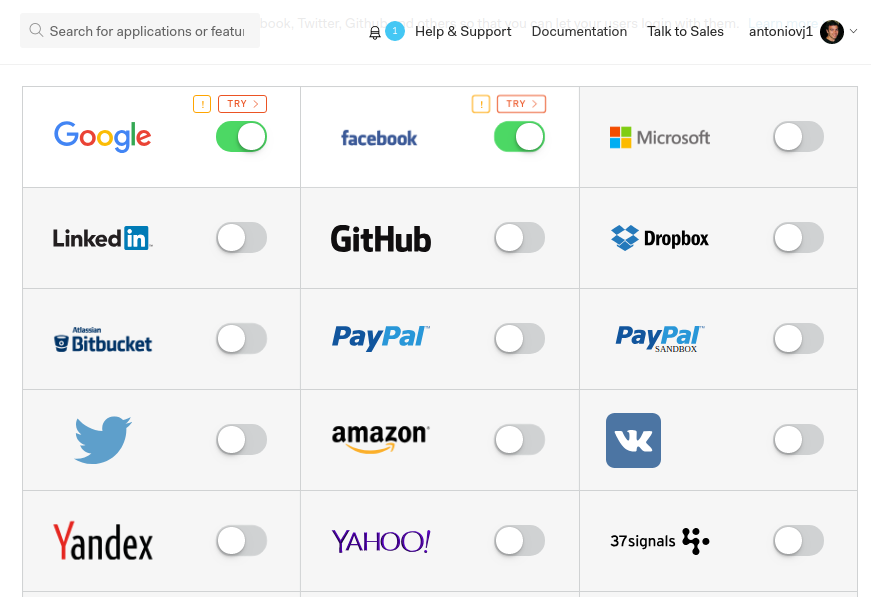
\includegraphics[width=0.95\textwidth]{imagenes/auth0.png}
    \caption{Proveedores de identidad Auth0}
    \label{fig:auth0}
  \end{center}
\end{figure}

\subsection {Bases de datos}
En esta sección se comentaré uno de los grandes motivos por los que decidimos el uso de una base de datos No-SQL, MongoDB. En un principio, no sabia exactamente que datos debía almacenar, y ademas era consciente de que a lo largo del tiempo los esquemas deberían evolucionar para proporcionar nueva información. Pensando en la implementación con una base de datos SQL y tras hacer algunas pruebas, comprobé que definir unos esquemas, añadir datos y a posteriori añadir nuevas columnas al esquema o eliminar alguna de las existentes parecía una tarea bastante tediosa y por ello decidimos optar por una solución mas flexible, en la que modificar los esquemas consistiera en realizar simples modificaciones en nuestro código y olvidarnos de migraciones.

\subsection {Ecosistema de React}
El principal problema encontrado, no ha sido a nivel de código, si no a nivel de gestión de dependencias. React solo proporciona algunas funciones básicas para la gestión de los componentes y su estado. Conforme queremos ir realizando mas operaciones, debemos ir añadiendo paquetes de NPM que nos den esa funcionalidad, de modo que en este proyecto encontramos un total de 78 dependencias, de las cuales 21 son para el desarrollo. Para cada nueva funcionalidad existe numerosas alternativas y numerosas versiones en constante cambio, lo cual crea una gran dificultad para elegir y una gran inversión de tiempo en lectura de documentación para averiguar cual se ajusta mejor a nuestro problema, además de las posibles incompatibilidades de versiones entre unos paquetes y otros. Para ilustrar la complejidad, cabe decir que actualmente existen mas de 700000 paquetes en NPM.

\subsection {Hot Module Replacement}
Durante la fase de desarrollo es interesante poder visualizar los cambios con la mayor agilidad posible, en principio mediante el uso de webpack y su opción de monitorización era posible recompilar la aplicación completa con cada cambio realizado. Esto suponía dos problemas, en primer lugar, era lento, y en segundo lugar, en cada recarga se perdía el estado de la pantalla debido a la recarga. Para subsanar esta situación se hizo uso de una técnica llamada HMR (Hot Module Replacement), con la cual tras añadir una serie de configuraciones y solventar los conflictos que generaba con la configuración te test, fuimos capaces de recompilar solo las partes afectadas por los cambios y mostrarlas sin necesidad de recargar el navegador y aun más importante, sin perder el estado.










%
\chapter{Pruebas}

En el capítulo anterior, se proporcionaba una visión sobre la implementación realizada, en este capítulo procederemos a mostrar que todo lo implementado se encuentra en funcionamiento.

\section {Pruebas unitarias}
Para la realización de las pruebas unitarias hemos hecho uso de Jest, una suite de test que integra numerosas herramientas. Para llevar a cabo la ejecución de los test usaremos la orden npm test, que ejecutará todos los archivos *.test.js. Dentro de estos archivos encontramos una líneas que indican los nombres de los tests (describe) y una serie de líneas que empiezan con la función test, dentro de las cuales se ejecutan y se evalúan las pruebas definidas.

Una vez ejecutamos los test obtendremos una serie de salidas, en las cuales se indica el éxito o el fallo de los test, y además en caso de fallo, se incluye una descripción de cuál ha sido la causa de este.
\begin{figure}
  \begin{center}
    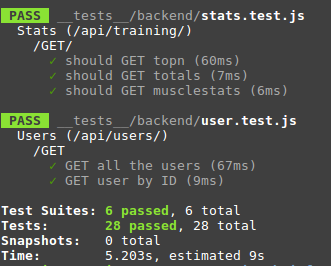
\includegraphics[width=\textwidth]{imagenes/test_pass.png}
    \caption{}
    \label{fig:}
  \end{center}
\end{figure}
\begin{figure}
  \begin{center}
    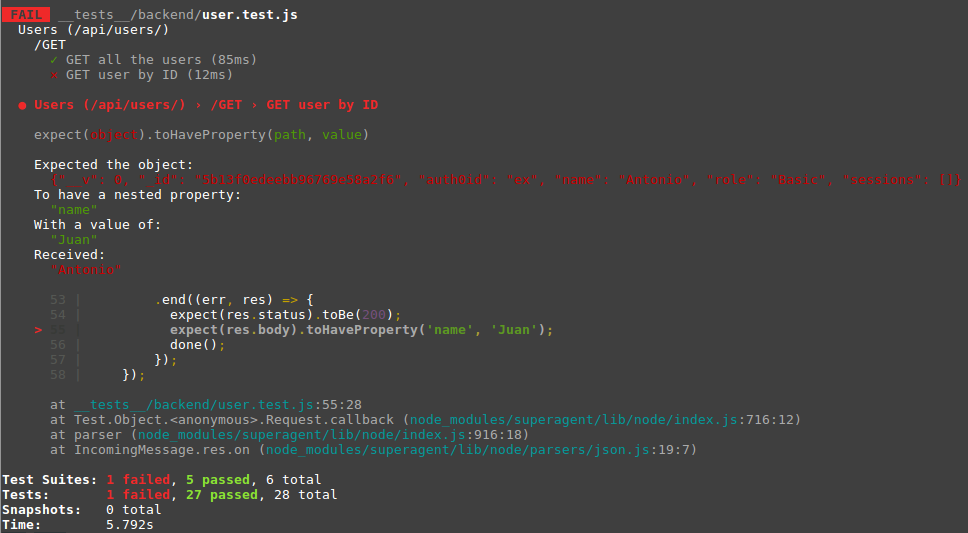
\includegraphics[width=\textwidth]{imagenes/test_fail.png}
    \caption{}
    \label{fig:}
  \end{center}
\end{figure}
\section {Pruebas de cobertura}
Para las pruebas de cobertura también se ha hecho uso de Jest. Para la ejecución de estas pruebas hacemos uso de la orden npm run test-cov, esta ejecución consiste en realizar los test anteriores y comprobar que líneas ha sido cubiertas por ellos. Una vez finalizada la ejecución, se proporciona un resumen por pantalla y además se genera un informe mucho más detallado en formato HTML , en el cual podremos ver con todo lujo de detalles cuáles líneas han sido testeadas y cuáles de ellas no.

\begin{figure}
  \begin{center}
    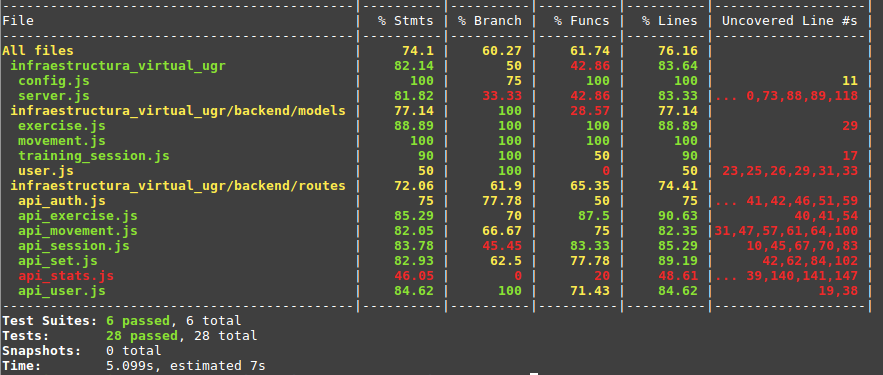
\includegraphics[width=\textwidth]{imagenes/cov.png}
    \caption{}
    \label{fig:}
  \end{center}
\end{figure}
\begin{figure}
  \begin{center}
    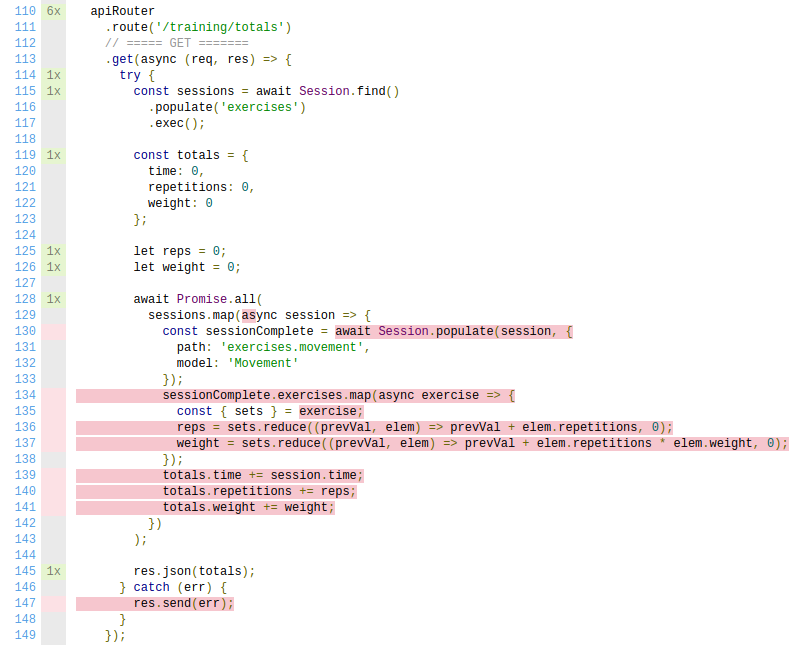
\includegraphics[width=\textwidth]{imagenes/cov_detail.png}
    \caption{}
    \label{fig:}
  \end{center}
\end{figure}

\section {Integración continua}
Una vez que disponemos de los test unitarios y nuestro archivo NPM tiene las órdenes indicadas para ejecutarlos, la integración con Travis CI es muy sencilla. Para comprobar que todo funciona como debe, nos dirigimos a la web de Travis, y hacemos un push al repositorio, tras lo que podremos observar que los test empiezan a ejecutarse, confirmando con ello la correcta configuración.

\begin{figure}
  \begin{center}
    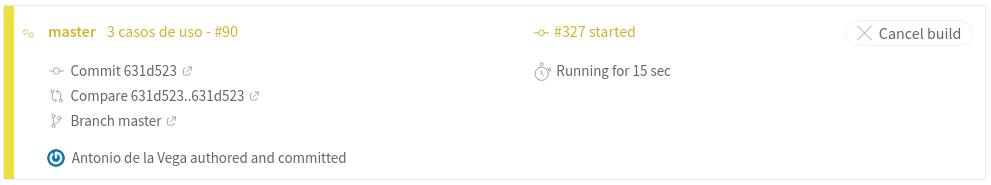
\includegraphics[width=\textwidth]{imagenes/init_travis.png}
    \caption{}
    \label{fig:}
  \end{center}
\end{figure}
\begin{figure}
  \begin{center}
    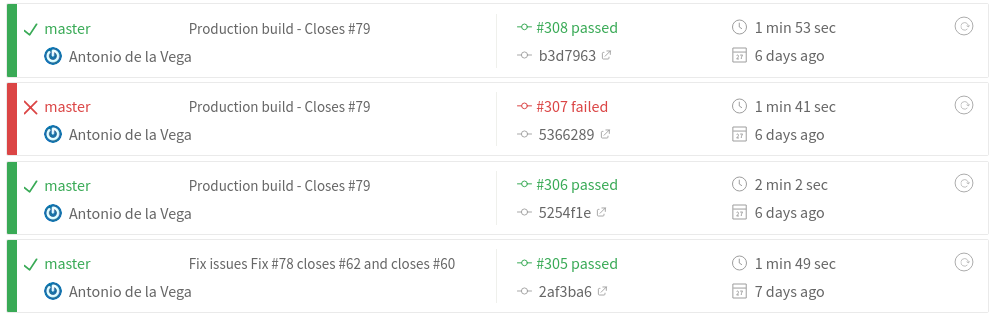
\includegraphics[width=\textwidth]{imagenes/travis.png}
    \caption{}
    \label{fig:}
  \end{center}
\end{figure}


\section {Despliegue automático}
Para el despliegue automático hemos hecho uso de Heroku, y con el objetivo de comprobar que todo está configurado de la forma correcta, nos dirigimos a la correspondiente web. Una vez ahí, hacemos un push a nuestro repositorio, y tras esperar a que Travis CI verifique los test, comenzamos a ver cómo se produce un nuevo build y seguidamente un nuevo despliegue, confirmando así que todo funciona de manera adecuada.


\begin{figure}
  \begin{center}
    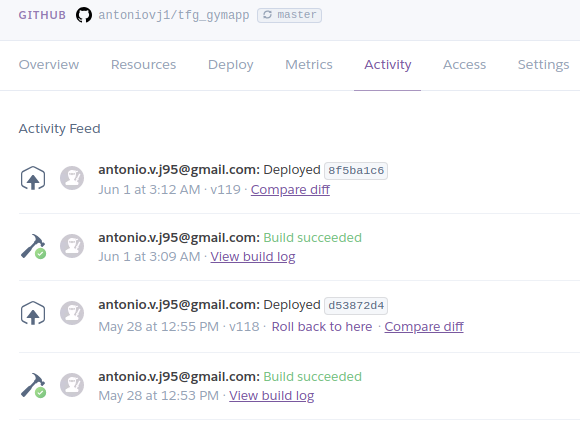
\includegraphics[width=\textwidth]{imagenes/heroku.png}
    \caption{}
    \label{fig:}
  \end{center}
\end{figure}

\section {Contenedores}
También hemos comprobado que los contenedores se ejecutan correctamente, y a continuación en la figura, se muestra como comienza la ejecución sin errorres.
\begin{figure}
  \begin{center}
    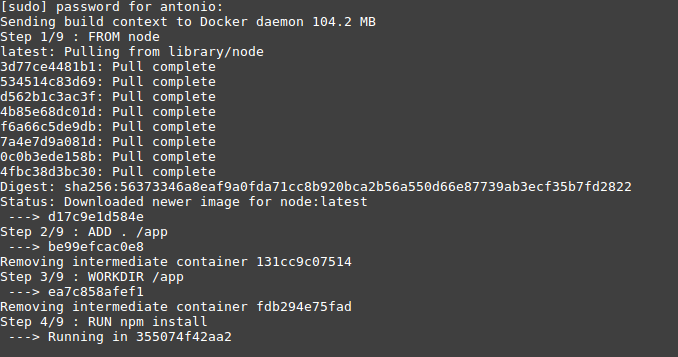
\includegraphics[width=\textwidth]{imagenes/docker.png}
    \caption{}
    \label{fig:}
  \end{center}
\end{figure}
\section {Provisionamiento}
\section {Despliegue Cloud}
\section {Acceso web y autenticación}

%
\chapter{Conclusiones}

Tras la realización de este proyecto, he adquirido grandes conocimientos en programación asíncrona, debido al comportamiento de Node y de las peticiones HTTP. Siendo concreto, debido a al funcionamiento de JavaScript, he aprendido a trabajar con promesas y las correspondientes funciones para crearlas y manejarlas, como pueden ser them, Async/Await... Además de eso he conseguido una comprensión más profunda del funcionamiento HTTP, por el desarrollo de la API, de las bases de datos No-SQL y el funcionamiento del DOM y las ventajas que aporta React en su manipulación.

Cabe destacar que debido a la gran cantidad de herramientas utilizadas, la puesta en marcha del desarrollo ha sido un tanto lenta, que debido a la naturaleza continua del desarrollo, las fases análisis y planificación han sido algo complejas, pero esto se compensa debido a la ayuda que dichas herramientas proporcionan para crear un código de calidad, modular y reutilizable.

El futuro del proyecto tiene dos claros frentes, en primer lugar mejorar los test y en segundo lugar, hacer uso de los datos almacenados.
\begin{itemize}
  \item \textbf{Mejorar los tests: } El primer objetivo a complir es añadir tests para el frontend y mejorar los ya existentes. Además se buscará incrementar la cobertura lo maximo posible, pero sin desperdiciar mucho tiempo en ello, ya que lo realmente importante es tener uns test de calidad, se puede tener una cobertura del 100\% y no por ello obtener un mejor código, con lo cual tampoco deberemos invertir más recursos de los necesarios en mejorar esa cifra. Por ello, lo importante será una gran cobertura de funcionalidades, pero no necesariamente de líneas de código.
  \item \textbf{Explotación de datos: } El siguiente paso lógico en el desarrollo, es hacer un uso intensivo de los datos almacenados, por un lado mostrando una pestaña de análisis con funciones más avanzadas, y por otro lado, con ayuda de personas con conocimientos más avanzados en fisiología del ejercicio, tratar de proporcionar información útil a los usuarios, detectar posibles anomalías y mostrar las posibles causas de ellas así como algunos consejos para afrontarlas.
\end{itemize}

Como conclusión me gustaría remarcar que el proyecto queda completamente libre, y que espero sea de utilidad a personas que quieran iniciarse en el desarrollo Full Stack, así como en el uso de herramientas para integración continua, despliegue continuo, verificación de calidad del código, infraestructura virtual...



%
  
\nocite{*}

\printglossaries

\begin{appendices}
\advance\csname @enumdepth\endcsname\csname @ne\endcsname
\section{Creative Commons Legal Code}

\subsection{Attribution-ShareAlike 4.0 International}



Official translations of this license are available in other languages.



\par Creative Commons Corporation (“Creative Commons”) is not a law firm and does not provide legal services or legal advice. Distribution of Creative Commons public licenses does not create a lawyer-client or other relationship. Creative Commons makes its licenses and related information available on an “as-is” basis. Creative Commons gives no warranties regarding its licenses, any material licensed under their terms and conditions, or any related information. Creative Commons disclaims all liability for damages resulting from their use to the fullest extent possible.


\par \textbf{Using Creative Commons Public Licenses}
\par Creative Commons public licenses provide a standard set of terms and conditions that creators and other rights holders may use to share original works of authorship and other material subject to copyright and certain other rights specified in the public license below. The following considerations are for informational purposes only, are not exhaustive, and do not form part of our licenses.
\begin{quotation}\textbf{Considerations for licensors:} Our public licenses are intended for use by those authorized to give the public permission to use material in ways otherwise restricted by copyright and certain other rights. Our licenses are irrevocable. Licensors should read and understand the terms and conditions of the license they choose before applying it. Licensors should also secure all rights necessary before applying our licenses so that the public can reuse the material as expected. Licensors should clearly mark any material not subject to the license. This includes other CC-licensed material, or material used under an exception or limitation to copyright. More considerations for licensors.\end{quotation}
\begin{quotation}\textbf{Considerations for the public:} By using one of our public licenses, a licensor grants the public permission to use the licensed material under specified terms and conditions. If the licensor’s permission is not necessary for any reason–for example, because of any applicable exception or limitation to copyright–then that use is not regulated by the license. Our licenses grant only permissions under copyright and certain other rights that a licensor has authority to grant. Use of the licensed material may still be restricted for other reasons, including because others have copyright or other rights in the material. A licensor may make special requests, such as asking that all changes be marked or described. Although not required by our licenses, you are encouraged to respect those requests where reasonable.
More considerations for the public.\end{quotation}

\subsubsection{Creative Commons Attribution-ShareAlike 4.0 International Public License}
\par By exercising the Licensed Rights (defined below), You accept and agree to be bound by the terms and conditions of this Creative Commons Attribution-ShareAlike 4.0 International Public License (``Public License''). To the extent this Public License may be interpreted as a contract, You are granted the Licensed Rights in consideration of Your acceptance of these terms and conditions, and the Licensor grants You such rights in consideration of benefits the Licensor receives from making the Licensed Material available under these terms and conditions.
\par \textbf{Section 1 – Definitions.}
\begin{enumerate}
\item \textbf{Adapted Material} means material subject to Copyright and Similar Rights that is derived from or based upon the Licensed Material and in which the Licensed Material is translated, altered, arranged, transformed, or otherwise modified in a manner requiring permission under the Copyright and Similar Rights held by the Licensor. For purposes of this Public License, where the Licensed Material is a musical work, performance, or sound recording, Adapted Material is always produced where the Licensed Material is synched in timed relation with a moving image.
\item \textbf{Adapter's License} means the license You apply to Your Copyright and Similar Rights in Your contributions to Adapted Material in accordance with the terms and conditions of this Public License.
\item \textbf{BY-SA Compatible License} means a license listed at  creativecommons.org/compatiblelicenses, approved by Creative Commons as essentially the equivalent of this Public License.
\item \textbf{Copyright and Similar Rights} means copyright and/or similar rights closely related to copyright including, without limitation, performance, broadcast, sound recording, and Sui Generis Database Rights, without regard to how the rights are labeled or categorized. For purposes of this Public License, the rights specified in Section 2(b)(1)-(2) are not Copyright and Similar Rights.
\item \textbf{Effective Technological Measures} means those measures that, in the absence of proper authority, may not
be circumvented under laws fulfilling obligations under Article 11 of the WIPO Copyright Treaty adopted on December 20, 1996, and/or similar
international agreements.
\item \textbf{Exceptions and Limitations} means fair use, fair dealing, and/or any other exception or limitation to Copyright and Similar Rights that applies to Your use of the Licensed Material.
\item \textbf{License Elements} means the license attributes listed in the name of a Creative Commons Public License. The License Elements of this Public License are Attribution and ShareAlike.
\item \textbf{Licensed Material} means the artistic or literary work, database, or other material to which the Licensor applied this Public License.
\item \textbf{Licensed Rights} means the rights granted to You subject to the terms and conditions of this Public License, which are limited to all Copyright and Similar Rights that apply to Your use of the Licensed Material and that the Licensor has authority to license.
\item \textbf{Licensor} means the individual(s) or entity(ies) granting rights under this Public License.
\item \textbf{Share} means to provide material to the public by any means or process that requires permission under the Licensed Rights, such as reproduction, public display, public performance, distribution, dissemination, communication, or importation, and to make material available to the public including in ways that members of the public may access the material from a place and at a time individually chosen by them.
\item \textbf{Sui Generis Database Rights} means rights other than copyright resulting from Directive 96/9/EC of the European Parliament and of the Council of 11 March 1996 on the legal protection of databases, as amended and/or succeeded, as well as other essentially equivalent rights anywhere in the world.
\item \textbf{You} means the individual or entity exercising the Licensed Rights under this Public License. \textbf{Your} has a corresponding meaning.
\end{enumerate}
\par \textbf{Section 2 – Scope.}
\begin{enumerate}
\item \textbf{License grant}.
\begin{enumerate}
\item Subject to the terms and conditions of this Public License, the Licensor hereby grants You a worldwide, royalty-free, non-sublicensable, non-exclusive, irrevocable license to exercise the Licensed Rights in the Licensed Material to:
\begin{enumerate}
\item reproduce and Share the Licensed Material, in whole or in part; and
\item produce, reproduce, and Share Adapted Material.
\end{enumerate}
\item Exceptions and Limitations. For the avoidance of doubt, where Exceptions and Limitations apply to Your use, this Public License does not apply, and You do not need to comply with its terms and conditions.
\item Term. The term of this Public License is specified in Section 6(a).
\item Media and formats; technical modifications allowed. The Licensor authorizes You to exercise the Licensed Rights in all media and formats whether now known or hereafter created, and to make technical modifications necessary to do so. The Licensor waives and/or agrees not to assert any right or authority to forbid You from making technical modifications necessary to exercise the Licensed Rights, including technical modifications necessary to circumvent Effective Technological Measures. For purposes of this Public License, simply making modifications authorized by this Section 2(a)(4) never produces Adapted Material.
\item Downstream recipients.

\begin{enumerate}
\item Offer from the Licensor – Licensed Material. Every recipient of the Licensed Material automatically receives an offer from the Licensor to exercise the Licensed Rights under the terms and conditions of this Public License.
\item Additional offer from the Licensor – Adapted Material. Every recipient of Adapted Material from You automatically receives an offer from the Licensor to exercise the Licensed Rights in the Adapted Material under the conditions of the Adapter’s License You apply.
\item No downstream restrictions. You may not offer or impose any additional or different terms or conditions on, or apply any Effective Technological Measures to, the Licensed Material if doing so restricts exercise of the Licensed Rights by any recipient of the Licensed Material.
\end{enumerate}

\item No endorsement. Nothing in this Public License constitutes or may be construed as permission to assert or imply that You are, or that Your use of the Licensed Material is, connected with, or sponsored, endorsed, or granted official status by, the Licensor or others designated to receive attribution as provided in Section 3(a)(1)(A)(i).
\end{enumerate}
\item \par \textbf{Other rights}.
\begin{enumerate}
\item Moral rights, such as the right of integrity, are not licensed under this Public License, nor are publicity, privacy, and/or other similar personality rights; however, to the extent possible, the Licensor waives and/or agrees not to assert any such rights held by the Licensor to the limited extent necessary to allow You to exercise the Licensed Rights, but not otherwise.
\item Patent and trademark rights are not licensed under this Public License.
\item To the extent possible, the Licensor waives any right to collect royalties from You for the exercise of the Licensed Rights, whether directly or through a collecting society under any voluntary or waivable statutory or compulsory licensing scheme. In all other cases the Licensor expressly reserves any right to collect such royalties.
\end{enumerate}

\end{enumerate}
\par \textbf{Section 3 – License Conditions.}
\par Your exercise of the Licensed Rights is expressly made subject to the following conditions.
\begin{enumerate}
\item \par \textbf{Attribution}.
\begin{enumerate}
\item \par If You Share the Licensed Material (including in modified form), You must:
\begin{enumerate}
\item retain the following if it is supplied by the Licensor with the Licensed Material:
\begin{enumerate}
\item identification of the creator(s) of the Licensed Material and any others designated to receive attribution, in any reasonable manner requested by the Licensor (including by pseudonym if designated);
\item a copyright notice;
\item a notice that refers to this Public License; 
\item a notice that refers to the disclaimer of warranties;
\item a URI or hyperlink to the Licensed Material to the extent reasonably practicable;
\end{enumerate}
\item indicate if You modified the Licensed Material and retain an indication of any previous modifications; and
\item indicate the Licensed Material is licensed under this Public License,
and include the text of, or the URI or hyperlink to, this Public
License.
\end{enumerate}

\item You may satisfy the conditions in Section 3(a)(1) in any reasonable manner based on the medium, means, and context in which You Share the Licensed Material. For example, it may be reasonable to satisfy the conditions by providing a URI or hyperlink to a resource that includes the required information.
\item If requested by the Licensor, You must remove any of the information required by Section 3(a)(1)(A) to the extent reasonably practicable.
\end{enumerate}

\item \textbf{ShareAlike}.
\par In addition to the conditions in Section 3(a), if You Share Adapted Material You produce, the following conditions also apply.
\begin{enumerate}
\item The Adapter’s License You apply must be a Creative Commons license with the same License Elements, this version or later, or a BY-SA Compatible License.
\item You must include the text of, or the URI or hyperlink to, the Adapter's License You apply. You may satisfy this condition in any reasonable manner based on the medium, means, and context in which You Share Adapted Material.
\item You may not offer or impose any additional or different terms or conditions on, or apply any Effective Technological Measures to, Adapted Material that restrict exercise of the rights granted under the Adapter's License You apply.
\end{enumerate}

\end{enumerate}
\par \textbf{Section 4 – Sui Generis Database Rights.}
\par Where the Licensed Rights include Sui Generis Database Rights that apply to Your use of the Licensed Material:
\begin{enumerate}
\item for the avoidance of doubt, Section 2(a)(1) grants You the right to extract, reuse, reproduce, and Share all or a substantial portion of the contents of the database;
\item if You include all or a substantial portion of the database contents in a database in which You have Sui Generis Database Rights, then the database in which You have Sui Generis Database Rights (but not its individual contents) is Adapted Material, including for purposes of Section 3(b); and
\item You must comply with the conditions in Section 3(a) if You Share all or a substantial portion of the contents of the database.
\end{enumerate}
For the avoidance of doubt, this Section 4 supplements and does not replace Your obligations under this Public License where the Licensed Rights include other Copyright and Similar Rights.
\par \textbf{Section 5 – Disclaimer of Warranties and Limitation of Liability.}
\begin{enumerate}
\item \textbf{Unless otherwise separately undertaken by the Licensor, to the extent possible, the Licensor offers the Licensed Material as-is and as-available, and makes no representations or warranties of any kind concerning the Licensed Material, whether express, implied, statutory, or other. This includes, without limitation, warranties of title, merchantability, fitness for a particular purpose, non-infringement, absence of latent or other defects, accuracy, or the presence or absence of errors, whether or not known or discoverable. Where disclaimers of warranties are not allowed in full or in part, this disclaimer may not apply to You.}
\item \textbf{To the extent possible, in no event will the Licensor be liable to You on any legal theory (including, without limitation, negligence) or otherwise for any direct, special, indirect, incidental, consequential, punitive, exemplary, or other losses, costs, expenses, or damages arising out of this Public License or use of the Licensed Material, even if the Licensor has been advised of the possibility of such losses, costs, expenses, or damages. Where a limitation of liability is not allowed in full or in part, this limitation may not apply to You.}
\end{enumerate}
\begin{enumerate}
\item The disclaimer of warranties and limitation of liability provided above shall be interpreted in a manner that, to the extent possible, most closely approximates an absolute disclaimer and waiver of all liability.
\end{enumerate}
\par \textbf{Section 6 – Term and Termination.}
\begin{enumerate}
\item This Public License applies for the term of the Copyright and Similar Rights licensed here. However, if You fail to comply with this Public License, then Your rights under this Public License terminate automatically.
\item 
\par Where Your right to use the Licensed Material has terminated under Section 6(a), it reinstates:
\begin{enumerate}
\item automatically as of the date the violation is cured, provided it is cured within 30 days of Your discovery of the violation; or
\item upon express reinstatement by the Licensor.
\end{enumerate}
For the avoidance of doubt, this Section 6(b) does not affect any right the Licensor may have to seek remedies for Your violations of this Public License.
\item For the avoidance of doubt, the Licensor may also offer the Licensed Material under separate terms or conditions or stop distributing the Licensed Material at any time; however, doing so will not terminate this Public License.
\item Sections 1, 5, 6, 7, and 8 survive termination of this Public License.
\end{enumerate}
\par \textbf{Section 7 – Other Terms and Conditions.}
\begin{enumerate}
\item The Licensor shall not be bound by any additional or different terms or conditions communicated by You unless expressly agreed.
\item Any arrangements, understandings, or agreements regarding the Licensed Material not stated herein are separate from and independent of the terms and conditions of this Public License.
\end{enumerate}
\par \textbf{Section 8 – Interpretation.}
\begin{enumerate}
\item For the avoidance of doubt, this Public License does not, and shall not be interpreted to, reduce, limit, restrict, or impose conditions on any use of the Licensed Material that could lawfully be made without permission under this Public License.
\item To the extent possible, if any provision of this Public License is deemed unenforceable, it shall be automatically reformed to the minimum extent necessary to make it enforceable. If the provision cannot be reformed, it shall be severed from this Public License without affecting the enforceability of the remaining terms and conditions.
\item No term or condition of this Public License will be waived and no failure to comply consented to unless expressly agreed to by the Licensor.
\item Nothing in this Public License constitutes or may be interpreted as a limitation upon, or waiver of, any privileges and immunities that apply to the Licensor or You, including from the legal processes of any jurisdiction or authority.
\end{enumerate}
\par Creative Commons is not a party to its public licenses. Notwithstanding, Creative Commons may elect to apply one of its public licenses to material it publishes and in those instances will be considered the “Licensor.” The text of the Creative Commons public licenses is dedicated to the public domain under the CC0 Public Domain Dedication. Except for the limited purpose of indicating that material is shared under a Creative Commons public license or as otherwise permitted by the Creative Commons policies published at creativecommons.org/policies, Creative Commons does not authorize the use of the trademark “Creative Commons” or any other trademark or logo of Creative Commons without its prior written consent including, without limitation, in connection with any unauthorized modifications to any of its public licenses or any other arrangements, understandings, or agreements concerning use of licensed material. For the avoidance of doubt, this paragraph does not form part of the public licenses.\\\\
Creative Commons may be contacted at creativecommons.org.
\par Additional languages available: Bahasa Indonesia, Nederlands, norsk, suomeksi, te reo Māori, українська, 日本語. Please read the FAQ for more information about official translations. 


\advance\csname @enumdepth\endcsname-\csname @ne\endcsname

\end{appendices}

\chapter*{}


\begin{thebibliography}{99}
	\addcontentsline{toc}{chapter}{Bibliografía}

\subsubsection*{Bibliografía artículos:}

\bibitem{} ``React Stateless Functional Components: Nine Wins You Might Have Overlooked''. Cory House, 29/03/2016. \url{https://hackernoon.com/react-stateless-functional-components-nine-wins-you-might-have-overlooked-997b0d933dbc}
\bibitem{} ``React-redux 'connect' explained ''. Soham Kaman, 31/03/2017. \url{https://www.sohamkamani.com/blog/2017/03/31/react-redux-connect-explained/}
\bibitem{} ``The Definitive Guide for building REST APIs''. Cléber Zavadniak, 10/06/2017. \url{https://medium.com/clebertech-en/the-definitive-guide-for-building-rest-apis-f70d37b1d656}
\bibitem{} ``React Binding Patterns: 5 Approaches for Handling `this`''. Cory House, 17/08/2016. \url{https://medium.freecodecamp.org/react-binding-patterns-5-approaches-for-handling-this-92c651b5af56}
\bibitem{} ``How Virtual-DOM and diffing works in React''. Gethyl George Kurian, 24/01/2017. \url{https://medium.com/@gethylgeorge/how-virtual-dom-and-diffing-works-in-react-6fc805f9f84e}
\bibitem{} ``MongoDB Schema Design: Relationships.''. 	William Zola, 29/05/2014.\url{https://www.mongodb.com/blog/post/6-rules-of-thumb-for-mongodb-schema-design-part-1}
\bibitem{} ``MongoDB Schema Design: Two-way referencing and denormalization''. William Zola, 06/06/2014.\url{https://www.mongodb.com/blog/post/6-rules-of-thumb-for-mongodb-schema-design-part-2}
\bibitem{} ``MongoDB Schema Design: Your guide through the rainbow''. William Zola, 11/06/2014.\url{https://www.mongodb.com/blog/post/6-rules-of-thumb-for-mongodb-schema-design-part-3}
\bibitem{} ``The 100\% correct way to structure a React app (or why there’s no such thing)''.David Gilbertson, 01/10/2017. \url{https://hackernoon.com/the-100-correct-way-to-structure-a-react-app-or-why-theres-no-such-thing-3ede534ef1ed}
\bibitem{} ``ReactJS Authentication Tutorial''. Prosper Otemuyiwa, 21/02/2017.\url{https://auth0.com/blog/reactjs-authentication-tutorial/}
\bibitem{} ``You Don't Know JS (book series)''. Kyle Simpson, 01/03/2014. \url{https://github.com/getify/You-Dont-Know-JS}
\bibitem{} ``ES6 Promises: Patterns and Anti-Patterns''. Bobby Brennan, 25/09/2017. \url{https://medium.com/datafire-io/es6-promises-patterns-and-anti-patterns-bbb21a5d0918}
\bibitem{} ``Docker Networking- How to connect multiple containers''. Osita Chibuike, 16/11/2017. \url{https://dev.to/mozartted/docker-networking--how-to-connect-multiple-containers-7fl}
\bibitem{} ``The Anatomy of a JSON Web Token''. Chris Sevilleja, 22/01/2015. \url{https://scotch.io/tutorials/the-anatomy-of-a-json-web-token}
\bibitem{} ``IBM: Get a grip on your JavaScript application state''. David Geary, 18/07/2016. \url{https://www.ibm.com/developerworks/library/wa-manage-state-with-redux-p1-david-geary/index.html}
\bibitem{} ``Webpack & The Hot Module Replacement''. Rajaraodv, 24/04/2016. \url{https://medium.com/@rajaraodv/webpack-hot-module-replacement-hmr-e756a726a07}

\bigskip
\subsubsection*{Bibliografía software más consultada:}
\bibitem{NJS} {\tt Node.js}. \url{https://nodejs.org/api/}
\bibitem{NPM} {\tt NPM}. \url{https://docs.npmjs.com/}
\bibitem{TCI} {\tt Travis CI}. \url{http://docs.travis-ci.com/}
\bibitem{Jest}. {\tt Jest}.  \url{https://facebook.github.io/jest/}
\bibitem{ReactJS}. {\tt React.js}.  \url{https://reactjs.org/}
\bibitem{Auth0}. {\tt Auth0}.  \url{https://auth0.com/docs}
\bibitem{Express.js}. {\tt Express.js}.  \url{http://expressjs.com/es/}
\bibitem{Material-UI}. {\tt Material-UI}.  \url{https://material-ui.com/}
\bibitem{Redux}. {\tt Redux}.  \url{https://es.redux.js.org/}
\bibitem{React-Router}. {\tt React-Router}.  \url{https://reacttraining.com/react-router/core/guides/philosophy}
\bibitem{Webpack}. {\tt Webpack}. \url{https://webpack.js.org}


\bigskip
\subsubsection*{Otra bibliografía:}
\begin{itemize}
  \item Consultas puntuales a la documentación de todos los servicios y dependencias.
	\item Consultas puntuales a {\tt Stack OverFlow}.
	\item Material docente asignaturas de la \textbf{Universidad de Granada}.
\end{itemize}

\end{thebibliography}

\end{document}
